% Autor: Manuel Lippert
% Topic: Bachelor Thesis

% Main-File


% Packages
\documentclass[paper=a4,bibliography=totoc,BCOR=10mm,numbers=noenddot,fontsize=11pt,headsepline]{scrreprt}
\usepackage[english]{babel}
\usepackage[T1]{fontenc}
\usepackage[latin1, utf8]{luainputenc}        %ä, ö, ü included
\usepackage[babel,german=quotes]{csquotes} %Quotes
\usepackage{lmodern}
\usepackage{graphicx}
\usepackage{nicefrac}
\usepackage{fancyvrb}
\usepackage{amsmath,amssymb,amstext}
\usepackage{siunitx}
\usepackage{url}
\usepackage[numbers, super]{natbib}
\usepackage{microtype}
\usepackage[format=hang]{caption}
\usepackage{physics}
\usepackage{titleref} 

% Additional Packages
\usepackage{geometry}                      % Geometry
\usepackage{anyfontsize}                   % All font sizes
\usepackage[table]{xcolor}                 % Colors in tables
\usepackage{ifthen}                        % If then statements
\usepackage[absolute,overlay]{textpos}     % Text boxes
\usepackage{amsfonts}                      % Fonts
\usepackage{xstring}                       % String operations
\usepackage{tikz}                          % Drawings
\usepackage{pdfpages}                      % Import of pdfs
\usepackage[hidelinks]{hyperref}                      % Links in document
\usepackage{makecell}                      % New line in tables
\usepackage{rotating}
\usepackage{booktabs}

% Paragraph changes
\parindent 0.0cm
\parskip 0.8ex plus 0.5ex minus 0.5ex

% Count and size of float objects
% maximal 2 in top and bottom big pictures also possible
\setcounter{bottomnumber}{2}
\setcounter{topnumber}{2}
\renewcommand{\bottomfraction}{1.}
\renewcommand{\topfraction}{1.}
\renewcommand{\textfraction}{0.}

%\sc und \bc outdated
\DeclareOldFontCommand{\sc}{\normalfont\scshape}{\@nomath\sc}
\DeclareOldFontCommand{\bf}{\normalfont\scshape}{\textbf}

% Various
\pagestyle{headings}            
\graphicspath{{./Pictures/}}    % Path for pictures
\VerbatimFootnotes              % \verb etc. in \footnotes

% Functions
\newcommand\tab[1][1cm]{\hspace*{#1}}
\newcommand{\vect}[1]{\boldsymbol{\mathbf{#1}}}
\newcolumntype{g}{>{\columncolor[rgb]{ .741,  .843,  .933}}l}

\begin{document}

    \nonfrenchspacing

    % 0.Chapter Cover
    % 0. Cover

% Hier sind nur die Variablen und der Abschnitt Informationen (unten) zu bearbeiten der REst läuft automatisch ab (z.b Farbenänderung)

% Noch abänderbar nur ein Vorschlag
\newgeometry{top=30mm, bottom=20mm, inner=20mm, outer=20mm}
\thispagestyle{empty}

% Colors (Notability Colors)
\definecolor{Notablue}{HTML}{3498DB}		
\definecolor{Notared}{HTML}{CF366C}			
\definecolor{Notagreen}{HTML}{19B092}		
\definecolor{Notaorange}{HTML}{FA9D00}		
\definecolor{Notagrey}{HTML}{969696}		
\definecolor{Notalavendel}{HTML}{9DBBD8}	

% Boolean by default false. Für Absatz in der Überschrift
\newboolean{twoRows}
\newboolean{symbol}

% Funktions
\makeatletter
   \def\vhrulefill#1{\leavevmode\leaders\hrule\@height#1\hfill \kern\z@}
\makeatother
\newcommand*\ruleline[1]{\par\noindent\raisebox{.8ex}{\makebox[\linewidth]{\vhrulefill{\linethickness}\hspace{1ex}\raisebox{-.8ex}{#1}\hspace{1ex}\vhrulefill{\linethickness}}}}

% Variables
\def\schriftgrosse{30}
\def\linethickness{1,5pt}

\def\farbe{black}
\def\fach{PPD}
\def\name{Manuel Lippert - Paul Schwanitz}
\def\titel{Dünnfilmprozessierungstechniken \\[0,5cm] und \\[0,5cm] Filmhomogenität} % Absatz mit \\[0,5cm]
\def\bottom{SS2023}
\def\datum{28.03.2023}
\def\platz{Chemie- und Charakterisierungslaber der Gruppe Herzig}
\def\betreuer{Fabian Eller}

% Für Fortgeschrittenen Praktikum siehe unten
\def\teilnehmerm{Manuel Lippert}
\def\emailm{Manuel.Lippert@uni-bayreuth.de}
\def\teilnehmerp{Paul Schwanitz}
\def\emailp{Paul.Schwanitz@uni-bayreuth.de}

% Für Grundpraktikum siehe unten
\def\auswertp{Teilnehmer1}
\def\messp{Teilnehmer2}
\def\protop{Teilnehmer3}

\def\groupnr{1}

\begin{titlepage}
			
	\centering
	{\LARGE \sffamily {\textbf{\bottom}\par}}
	\vspace{2,5cm}
    {\fontsize{30}{0}\sffamily\ruleline{\textcolor{\farbe}{\textbf{\fach}}}\par}
    \vspace{6cm}
	{\Large\sffamily \ruleline{\name}\par}
		
	\IfSubStr {\titel} {\\[0,5cm]} {\setboolean{twoRows}{true}} {\setboolean{twoRows}{false}}
	
	\ifthenelse{\boolean{twoRows}}
		{
			\begin{textblock*}{21cm}(0cm,8cm) % {block width} (coords), centered		
				{\fontsize{\schriftgrosse}{0}\sffamily\textcolor{\farbe}{\textbf{\titel}}\par}
			\end{textblock*}
		}
		{
			\begin{textblock*}{21cm}(0cm,9cm) % {block width} (coords), centered		
				{\fontsize{\schriftgrosse}{0}\sffamily\textcolor{\farbe}{\textbf{\titel}}\par}
			\end{textblock*} 
		}
	
	% Choose Logo
	\ifthenelse {\equal{\farbe}{Notared}} {\def\logo{Bilder/Logo/UniBTNotared}}
		{\ifthenelse {\equal{\farbe}{Notagreen}} {\def\logo{Bilder/Logo/UniBTNotagreen}}
			{\ifthenelse {\equal{\farbe}{Notablue}} {\def\logo{Bilder/Logo/UniBTNotablue}}
				{\ifthenelse {\equal{\farbe}{Notaorange}} {\def\logo{Bilder/Logo/UniBTNotaorange}}
					{\ifthenelse {\equal{\farbe}{Notagrey}} {\def\logo{Bilder/Logo/UniBTNotagrey}}
						{\ifthenelse {\equal{\farbe}{Notalavendel}} {\def\logo{Bilder/Logo/UniBTNotalavendel}}	
							{\ifthenelse {\equal{\farbe}{black}} {\def\logo{Bilder/Logo/UniBT}}	
								{\def\logo{noLogo}}
							}
						}
					}
				}
			}
		}	

	\IfSubStr{\logo}{noLogo}{\setboolean{symbol}{false}}{\setboolean{symbol}{true}}
	
	% Gruppe
	\vspace{10cm}
	{\large\sffamily{Gruppe \groupnr}}
	
	%Logo
	\vfill

	\ifthenelse{\boolean{symbol}}
		{
			\begin{figure}[h]
			\begin{center}
				
				\includegraphics[width=2cm]{\logo}
				
			\end{center}
			\end{figure}
		}
	
\end{titlepage}

\restoregeometry

% Information
\chapter*{Informationen}
\label{chap:info}

\begin{tabular}{l l}

	{\textbf{Versuchstag}} \hspace{1cm} & \hspace{1cm} {\datum}\\[0,2cm]
	{\textbf{Versuchsplatz}} \hspace{1cm} & \hspace{1cm} {\platz}\\[0,2cm]
	{\textbf{Betreuer}} \hspace{1cm} & \hspace{1cm} {\betreuer}\\[1,2cm]
	{\textbf{Gruppen Nr.}} \hspace{1cm} & \hspace{1cm} {\groupnr}\\[0.2cm]
	% Für Fortgeschittenenen Praktikum
	{\textbf{Teilnehmer}} \hspace{1cm} & \hspace{1cm} {\teilnehmerm~(\emailm)}\\[0.2cm]
						  \hspace{1cm} & \hspace{1cm} {\teilnehmerp~(\emailp)}\\[0.2cm]
	% Für Grundpraktikum
	%{\textbf{Auswertperson}} \hspace{1cm} & \hspace{1cm} {\auswertp}\\[0.2cm]
	%{\textbf{Messperson}} \hspace{1cm} & \hspace{1cm} {\messp}\\[0.2cm]
	%{\textbf{Protokollperson}} \hspace{1cm} & \hspace{1cm} {\protop}\\[0.2cm]

\end{tabular}

    \thispagestyle{empty}
    \cleardoublepage
    \tableofcontents
    \cleardoublepage

    % 1.Chapter Instructions
    % 1. Introduction

\chapter{Introduction}
\label{chap:intro}

    % 2.Chapter Theorie
    \chapter{Theoretical background}
\label{chap:theory}

% text

\section{Singlet and Triplet Excited States}
\label{sec:excitedStates}

\begin{center}
    \captionsetup{type = figure}
    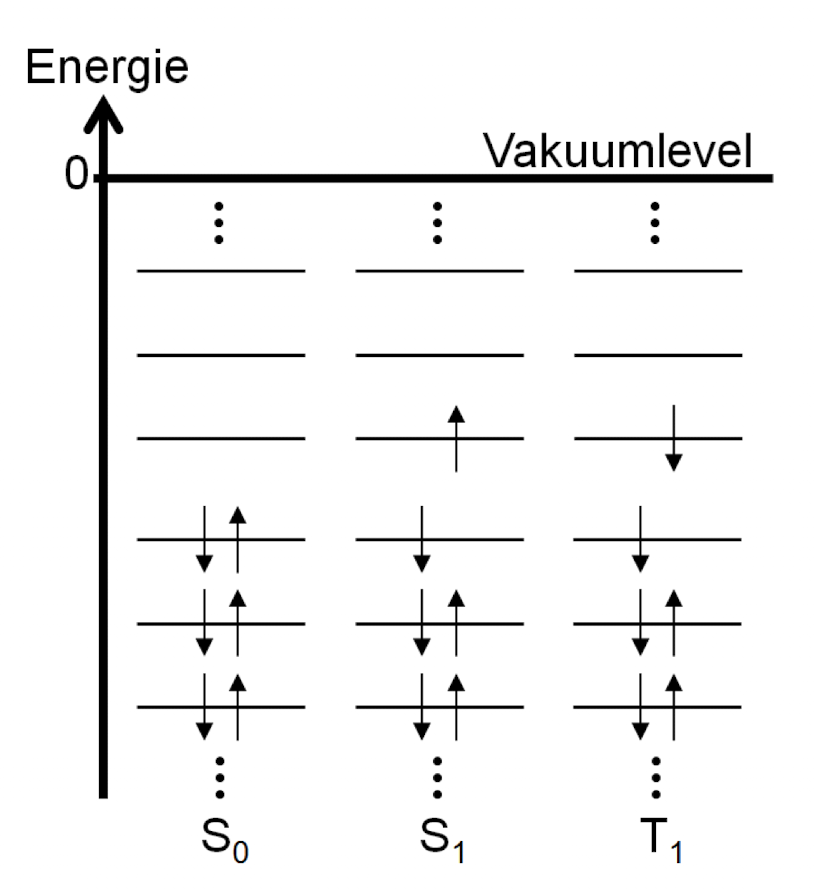
\includegraphics[width = 0.4\textwidth]{Pictures/Excited-States.png}
    \captionof{figure}{
        Orbital diagram of the dominant orbital occupations of the singlet states $S_0$ , $S_1$ and the triplet state $T_1$. \cite{Kilchert.04.2023} 
    }
    \label{fig:states}
\end{center}

In this section we want to discuss the relevant aspects of electronic processes in organic molecules. The energy levels of these systemes can be described by molecular orbitals. Molecular orbitals can be obtained through the usage of the \textbf{LCAO} method, which combines multiple atomic orbitals to a molecular orbital. A concrete occupation if these orbitals is called state, which have two specific states called \textbf{HOMO} (Highest Occupied Molecular Orbital) and \textbf{LOMO} (Lowest unOccupied Molecular Orbital). In addition to that distinction is made between singlet and triplet state with the following properties
\begin{itemize}
    \item Triplet State $T_i$: Total spin (sum of all electron spins) is $\pm 1$, 
    \item Singlet State $S_i$: Total spin is 0.
\end{itemize}
Figure \ref{fig:states} shows a simplified representation (only the largest contribution) of electronic states in molecules. 

\begin{center}
    \captionsetup{type = figure}
    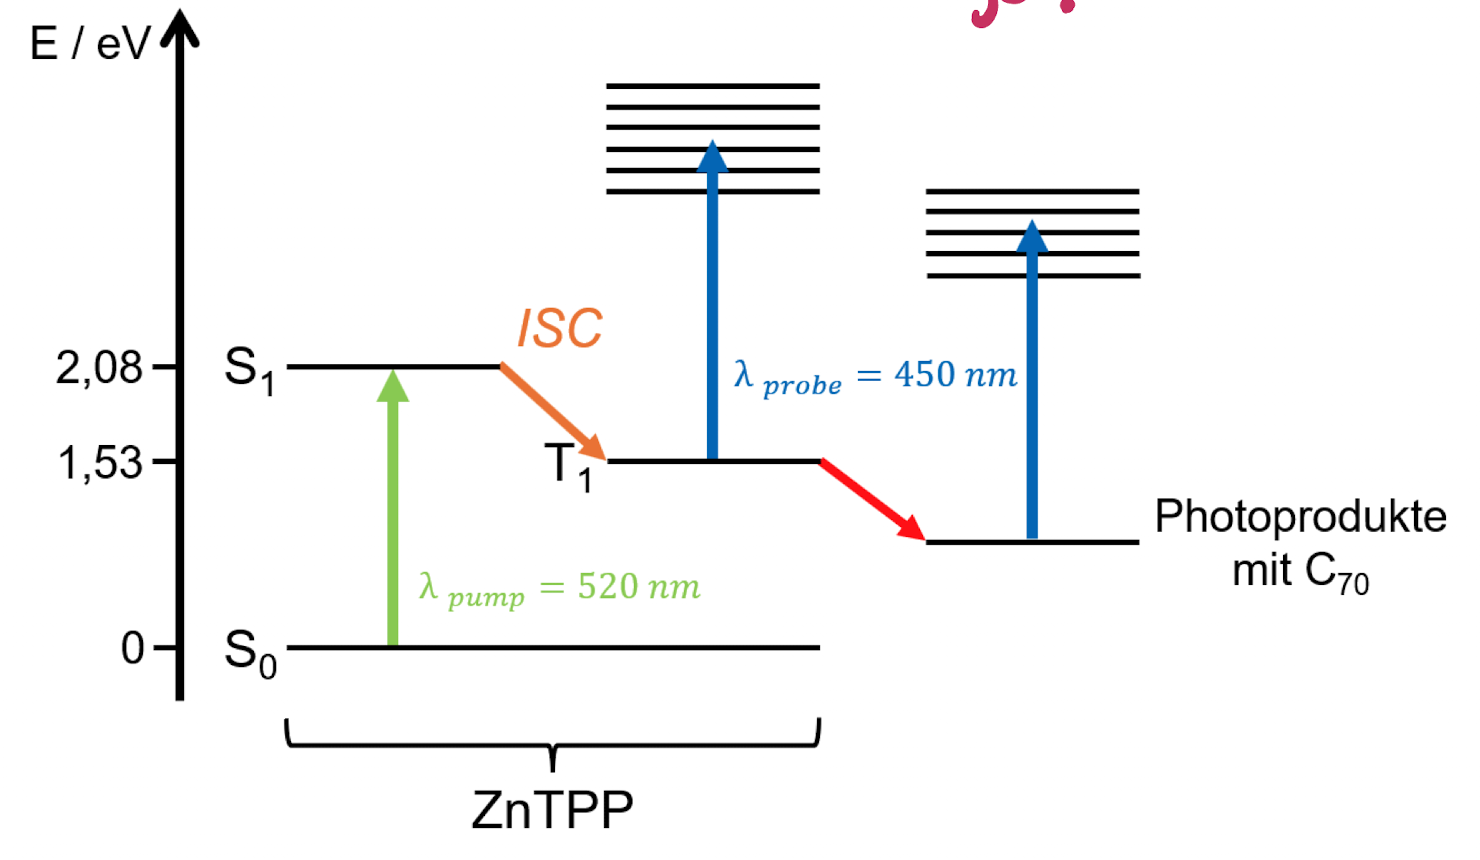
\includegraphics[width = 0.6\textwidth]{Pictures/Transition.png}
    \captionof{figure}{
        Jablonski scheme of the system of this experiment (ZnTPP and ZnTPP with fullerene $\mathrm{C}_{70}$). \cite{Kilchert.04.2023} 
    }
    \label{fig:transition}
\end{center}
To excite a system into from the ground state to the singlet state the system has to absorbe a photon with the energy corresponding to the transition, which leads to an absorption pattern the refelcts the structure of the energy levels of an atom. After absorption the electron relaxes back into the ground state (\textit{Kasha's Rule}). The transition can be radiative or non-radiative, but it is also possible to perform a transfer to a triplet state if the energy gap is small enough and one spin is flipped, which results in a sufficiently large spin-orbit coupling. The transition between singlet to triplet states is called Inter System Crossing (ISC). The jablonski scheme of this transition process for the relevant molecule of this experiment (ZnTPP and ZnTPP with fullerene $\mathrm{C}_{70}$) is shown in Figure \ref{fig:transition}. 
\bigskip

The radiative transition of an electron from the singlet state to the ground state is called \textbf{Flourescence} and from a triplet state to the ground state \textbf{Phosphorescence}. Both mentioned transitions are examples for \textit{radiative decays} with the emission of a photon. In case of ISC it is a \textit{non-radiative decay}, since the energy of the excited singlet state gets disspated due to ISC. The lifetime $\tau$ of the excited state will be given by the expression
\begin{gather}
    \tau = \frac{1}{k_\mathrm{r} + k_\mathrm{nr}},
\end{gather}
with the $k_\mathrm{r}$ and $k_\mathrm{nr}$ as the decay rates of the radiative and non-radiative decay. The determination is achieved by a pump-probe experiment, which will be discussed in Chapter \ref{sec:transient}. \cite{Kilchert.04.2023}
Scince the process of ISC is non-radiative one can not directly measure ISC, but if the energy level aif the singlet state is known and the decay rate of the triplet state will be measured, it is possible to indirectly measure the energy loss of ISC.
\newpage
\section{Transient Absorption Spectroscopy}
\label{sec:transient}

In this experiment different treatments were investigated in terms of lifetime $\tau$ of the solution itself. At the beginning we expect from theory that the decay of the concentration of the triplet state $C_\mathrm{T}(t)$ is exponential and given by the relation
\begin{gather}
    C_\mathrm{T}(t) = C_\mathrm{T}(0) e^{-k_0 t} + C_\mathrm{T}^\mathrm{Off}~,
    \label{eq:fitExp}
\end{gather}
with the initial concentration $C_\mathrm{T}$ and the decay rate $k_0$. Also, an offset concentration $C_\mathrm{T}^\mathrm{Off}$ was added to encounter any offset cuased by e.g. measuring methods. Since the transient absorption (TA) is porportional to $C_\mathrm{T}(t)$, we can fit the same exponential decay for the transient absorption as well. The full set of fitted treatments and results of the exponential fit can be found in Tab. \ref{tab:lifetimeDecay}. The lifetime $\tau$ was calculated with the relation $\tau = 1/k$. The exponential fits itself are displayed in Fig. \ref{fig:lifetimeDecay}\,.
\begin{center}
    \captionsetup{type = table}
    \begin{tabular}{| c | l | c c |}
        \hline
        No & Treatment             & $k_0$/ms$^{-1}$            & $\tau$/ns   \\\hline
        1  & ZnTPP in BN 0.8\,mM   & 1089 $\pm$ 4               & 919 $\pm$ 3 \\
        2  & ZnTPP in BN 0.6\,mM   & 1077 $\pm$ 5               & 929 $\pm$ 4 \\
        3  & ZnTPP in BN 0.4\,mM   & 1069 $\pm$ 5               & 936 $\pm$ 4 \\
        4  & ZnTPP in BN 0.2\,mM   & 1057 $\pm$ 8               & 946 $\pm$ 7 \\\hline
        8  & ZnTPP in Tol 0.8\,mM  & 1891 $\pm$ 3               & 529 $\pm$ 1 \\\hline
        12 & ZnOEP in BN 0.8\,mM   & 2681 $\pm$ 5               & 373 $\pm$ 1 \\\hline
        \multicolumn{4}{c}{}\\\hline
        No & Treatment             & $k_\mathrm{app}$/ms$^{-1}$ & $\tau$/ns   \\\hline
        5  & ZnTPP:C70 in BN 1:0.1 & 1254 $\pm$ 5               & 798 $\pm$ 3 \\
        6  & ZnTPP:C70 in BN 1:0.2 & 1385 $\pm$ 6               & 722 $\pm$ 3 \\
        7  & ZnTPP:C70 in BN 1:0.3 & 1436 $\pm$ 6               & 697 $\pm$ 3 \\\hline
    \end{tabular}
    \captionof{table}{
        Calculated decay rates $k_0$ and $k_\mathrm{app}$ and lifetimes $\tau$ ($\tau = 1/k$) for different types of treatments.
    }
    \label{tab:lifetimeDecay}
\end{center}

\subsection{Influence of Concentration}
\label{sub:concentration}

First, we want to investigate the influence of concentration on the deacy rate $k_0$, i.e., the lifetime $\tau$. For that we take a closer look at sample number $1-4$ [Tab. \ref{tab:lifetimeDecay}]. In Fig. \ref{fig:lifetimeDecay}\,(a) it is clear that higher maxima correspond with to higher concentration of ZnTPP, which aligns with our expectation that higher concentration leads to a greater amount of absorption. The lifetime $\tau$ on the other hand increases with the reduction of concentration, which follows the expectation from the theory. The kinetics iof the decay of the triplet state are described by the equation
\begin{gather}
    \frac{\mathrm{d}}{\mathrm{d}t} C_\mathrm{T} = -k_1 C_\mathrm{T}(t) - k_2(C_\mathrm{T}(t))^2 - k_3C_\mathrm{T}(t)C_\mathrm{G}(t)~,
    \label{eq:kineticsTriplet}
\end{gather}
where $C_\mathrm{G}(t)$ is the concentration of the ground state and $k_1, k_2, k_3$ are decay rates. In further calculation the assumption $C_\mathrm{T}(t) \ll C_\mathrm{G}(t)$ will be made, which leads to the discussed exponential decay [Eq. (\ref{eq:fitExp})]. But, this assumption gets less valid for an increasing population of triplet states, to the point at which one has to take the terms with $C_\mathrm{T}(t)$ into account. This results in higher decay rates $k_0$ and shorter lifetimes $\tau$ of the triplet states. The same behaviour can be identife to the cases of higher concentration of ZnTPP in BN and explains the kinetics of the decay process.

\subsection{Influence of Fullerene \boldmath{$\mathrm{C}_{70}$}}
\label{sub:fullerene}

In the next paragraph the impact of the fullerene $\mathrm{C}_{70}$ on the lifetime $\tau$ will be addressed. We consider for this analysis sample 1 (base solution) and $5-7$ [Tab. \ref{tab:lifetimeDecay}]. In Fig. \ref{fig:lifetimeDecay}\,(b) one can see that the decreases the higher the concentration of the fullerene $C_\mathrm{q}$ gets, introducing a quenching process. This result was expected, because in theory the decay rate $k_0$ gets expanded as
\begin{gather}
    k_0 \longrightarrow k_\mathrm{app} = k_0 + k_\mathrm{q}C_\mathrm{q}~,
    \label{eq:decayExpand}
\end{gather}
with the new decay rate $k_\mathrm{app}$ and the reaction rate of quenching process $k_\mathrm{q}$. The expansion of the decay rate $k_0$ leads to higher decay rates $k_\mathrm{app}$ ($k_\mathrm{q} > 0$), which leads to shorter lifetimes $\tau$. To determine the quenchning reaction rate $k_\mathrm{q}$, we take the calculated decay rates $k_\mathrm{app}$ and fit them against the concentration $C_\mathrm{q}$ [Eq. \ref{eq:decayExpand}]. For the decay rate $k_0$ the decay rate of the base solution (sample 1) will be used. From the slope of the linear fit one can calculate the quenchning reaction rate $k_\mathrm{q}$. The linear fit can be seen in Fig. \ref{fig:concentration}. 

\begin{center}
    \captionsetup{type = figure}
    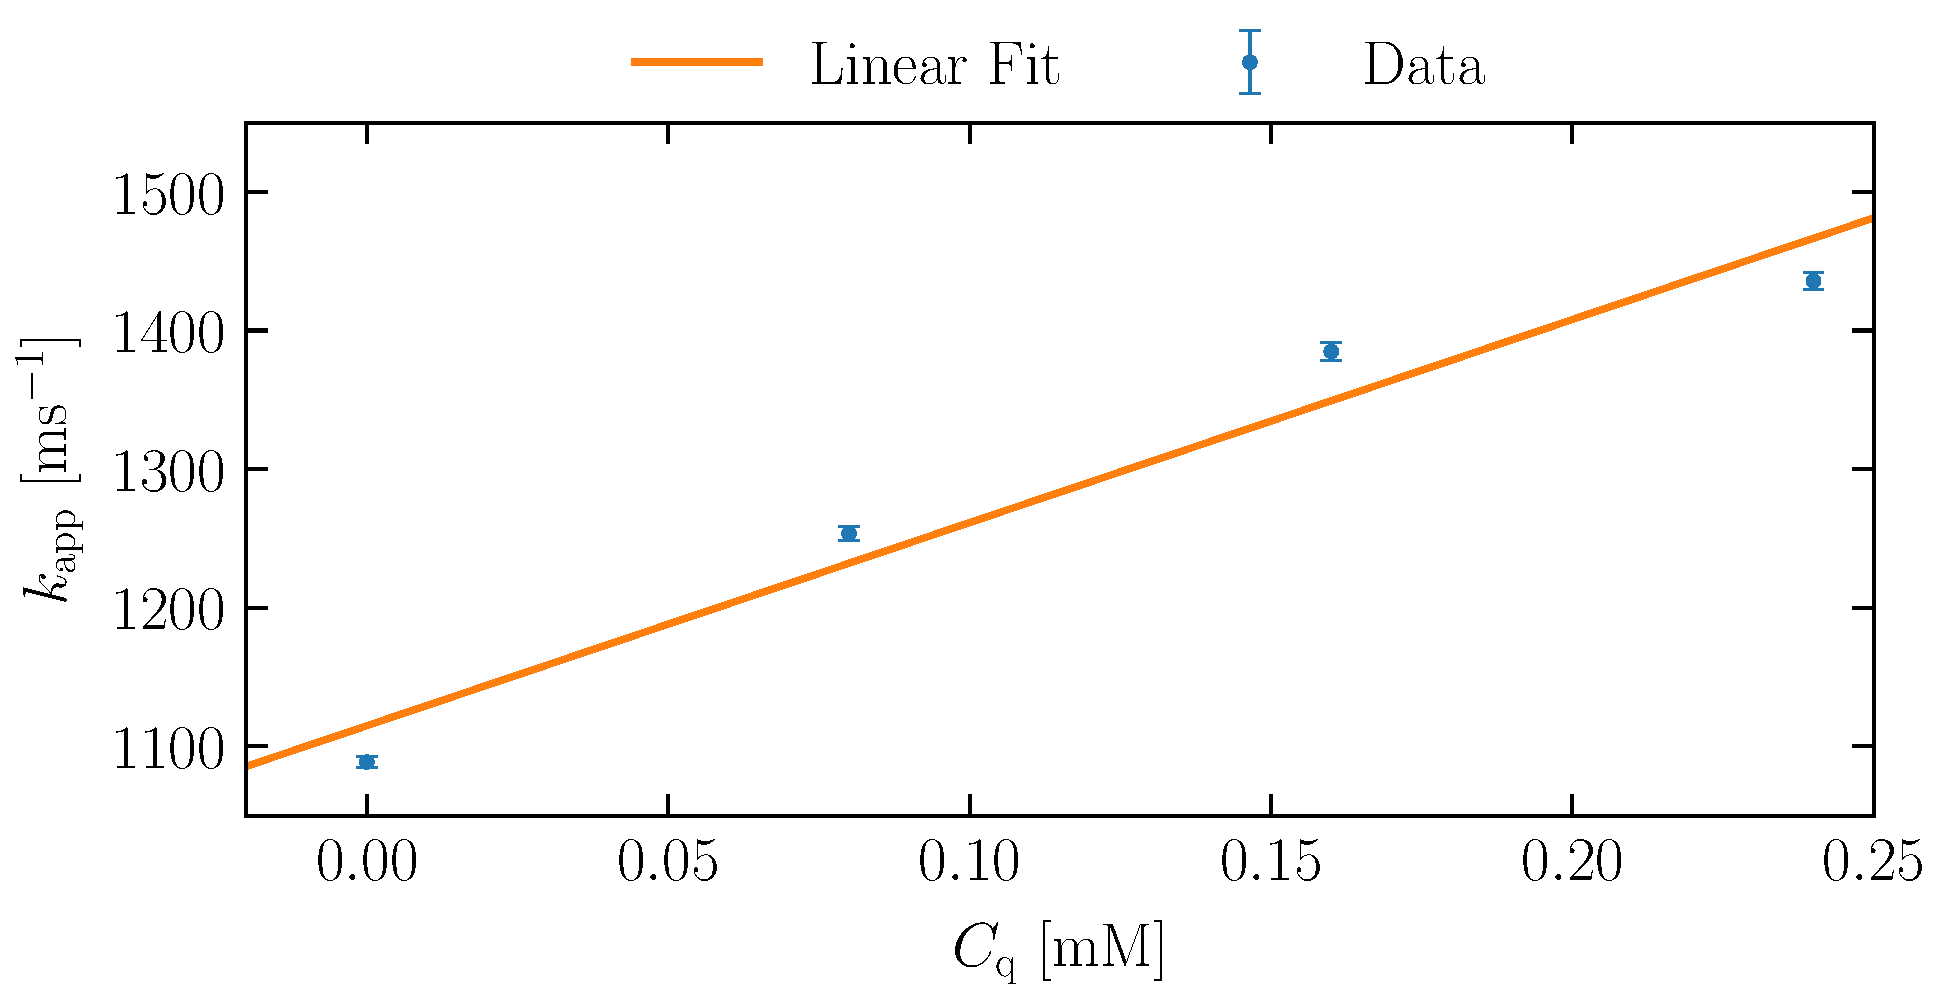
\includegraphics[width = 0.85\textwidth]{Pictures/Evaluation/42/Concentration.pdf}
    \captionof{figure}{
        Linear fit of decay rate $k_\mathrm{app}$ for different fullerene concentration $C_\mathrm{q}$. 
    }
    \label{fig:concentration}
\end{center}

The calculation yields
\begin{gather*}
    \boxed{k_\mathrm{q} = (1.5 \pm 0.2) \times 10^9\,\mathrm{sM^{-1}}}~, %1465.49 229.41 ms-1/mM
\end{gather*}
which does not align with the result of Ito et al.\cite{Nojiri.1998}, who determined $k_\mathrm{q} = 4.7 \times 10^9\,\mathrm{sM^{-1}}$, but is in the right order of magnitude.

\subsection{Influence of the Solvent}
\label{sub:difference}

In this paragraph the influence of Solvent on the transient absorption (TA) signal and the lifetime $\tau$ will be dicussed. 
\bigskip

First, we look at the variation of ZnTPP with BN and Tol for the concentration 0.8\,mM (sample 1 and 8 [Tab. \ref{tab:lifetimeDecay}]). In Fig. \ref{fig:lifetimeDecay}\,(c) we can observe the nearly same maximum value for both solutions but different lifetimes $\tau$, which are calculated in Tab. \ref{tab:lifetimeDecay}. This aligns with the UV-VIS spectroscopy from Chapter \ref{sec:uv-vis}, because the polarity of BN makes it easier to induce more charges into the delocalized $\pi$-electron system. So, it is possible to observe a redshift and an increase of lifetime $\tau$. 
\bigskip

Next, we vary the zinc complexes of the solution from ZnTPP to ZnOEP, but we keep BN as second solvent of the solution with concentration 0.8\,mM (sample 1 and 12 [Tab. \ref{tab:lifetimeDecay}]). The transient absorption signal can be found in Fig. \ref{fig:lifetimeDecay}\,(d) with the corresponding decay rates $k$ and lifetimes $\tau $ in Tab. \ref{tab:lifetimeDecay}. It is clearly visible that the maximum of the TA signal is for both zinc complexes the same but the lifetime $\tau$ for is much shorter for ZnOEP. The value of the TA maximum corresponds with the maximum concentration of the triplet state and is therefor correlated to the absorption of the pump laser light. Looking at the UV-VIS of ZnTPP and ZnOEP [Fig. \ref{fig:uv-visZinc}] one can conclude that the absorbance for ZnTPP and ZnOEP does not differ from each other, which explains teh same maximum value for the TA signal. The longer lifetime $\tau$ of ZnTPP can also be linked to the redshift compared to ZnOEP. Due to the four additional phenyl groups in ZnTPP, the conjugated electron system is bigger than in ZnOEP. So, a lower energy is needed to exite the electrons of ZnTPP.
\bigskip

Finally, we want to discuss the variation of the solution itself. For that, we take a look at sample 1 (ZnTPP in BN 0.8\,mM) and 9 (P3HT in Tol 1.5\,mM). In Fig. \ref{fig:difference} it is visible that P3HT has a smaller maximum compared to ZnTPP. From the previous lifetime analysis one can assume trivial that the lifetime of P3HT is shorter compared to the lifetime of ZnTPP. Comparing the UV-VIS of P3HT from Ref. \citenum{Rahimi2014} to the evaluation from ZnTPP from Chapter \ref{sec:uv-vis} the observed redshift is also present for P3HT as well as the smaller absorbance compared to ZnTPP. The underlying process relates to the P3HT aggregates, which can consist of crystalline regions, amorphous domains or a combination of both. Amorphous chain sequences lead to structural defects, grain boundaries and coiled-like chain conformations that can reduce intra-chain order. Therefore, UV-VIS absorption signatures are broadened and blue shifted towards higher energies \cite{Rahimi2014}, which results in the observed (TA) signal.

\begin{center}
    \captionsetup{type = figure}
    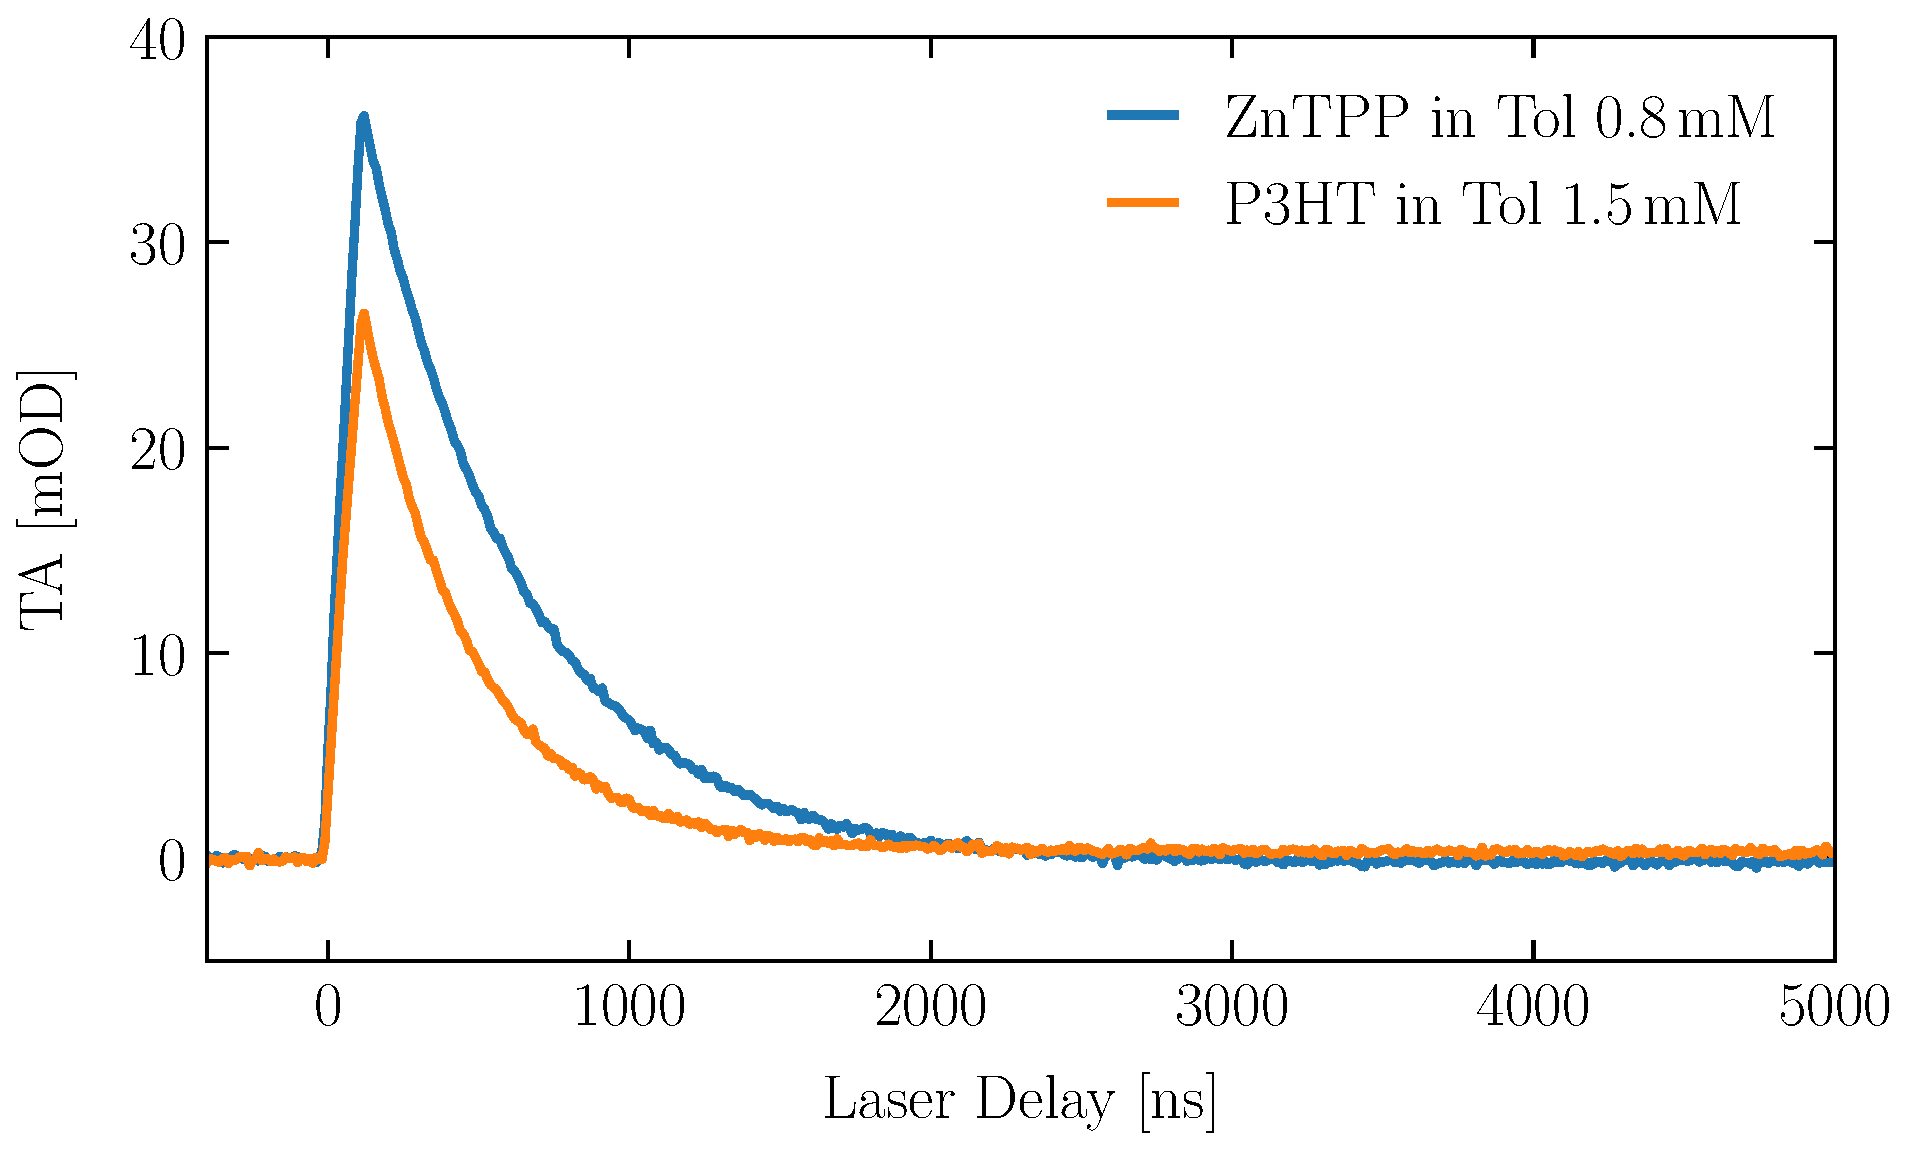
\includegraphics[width = 0.85\textwidth]{Pictures/Evaluation/42/Difference.pdf}
    \captionof{figure}{
        Transient absorption signal using different treatments with ZnTPP and P3HT 
    }
    \label{fig:difference}
\end{center}

\begin{center}
    \begin{sidewaysfigure}
    \centering
    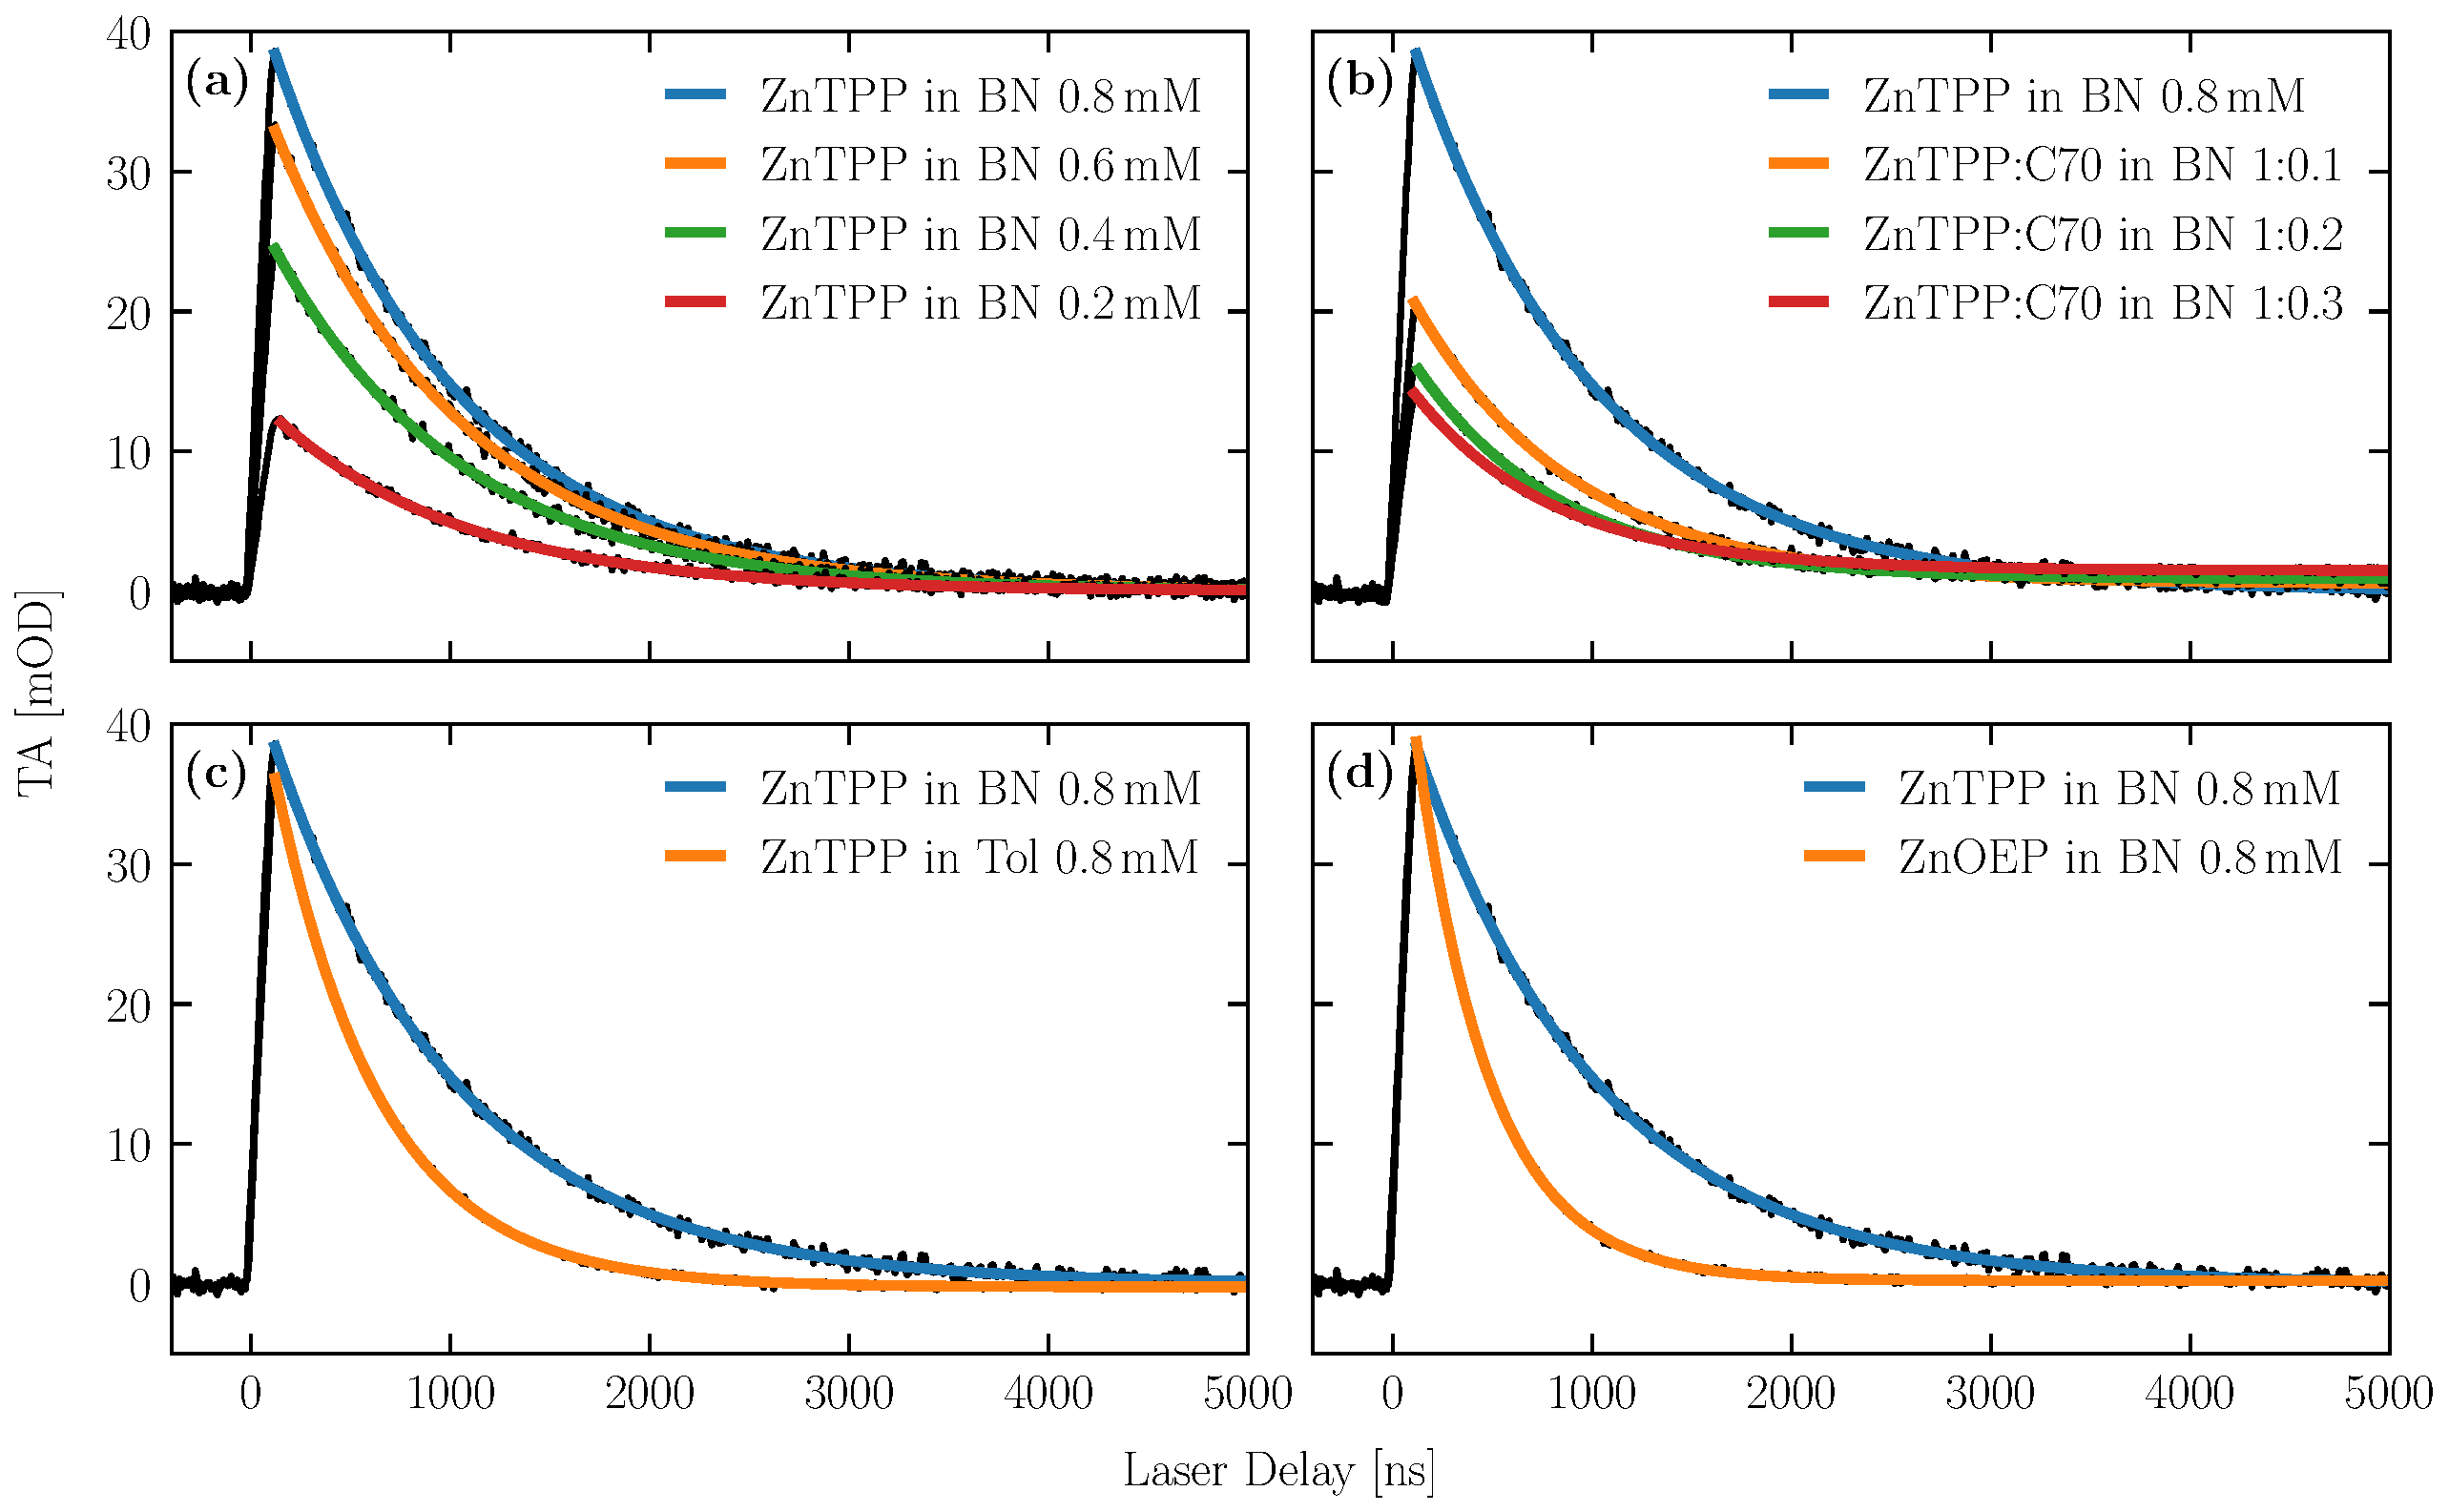
\includegraphics[width = 0.9\textheight]{Pictures/Evaluation/42/Lifetime.pdf}
    \caption{
        Comparison between data of the transient absorption of different treatments with the exponential fits colored for each treatment: (a) Different concentration of ZnTPP in BN, (b) Different dullutions of C$_{70}$ in ZnTPP in BN 0.8\,mnM, (c) Different Solvents (BN, Tol) with ZnTPP and a concentration of 0.8\,mM and (d) Different Solvents (ZnTPP, ZnOEP) with BN and a concentration of 0.8\,mM.
    }
    \label{fig:lifetimeDecay}
    \end{sidewaysfigure}
\end{center}
\newpage

\subsection{Influence of the Pump Laser Width}
\label{sub:pumpLaser}

\begin{center}
    \captionsetup{type = figure}
    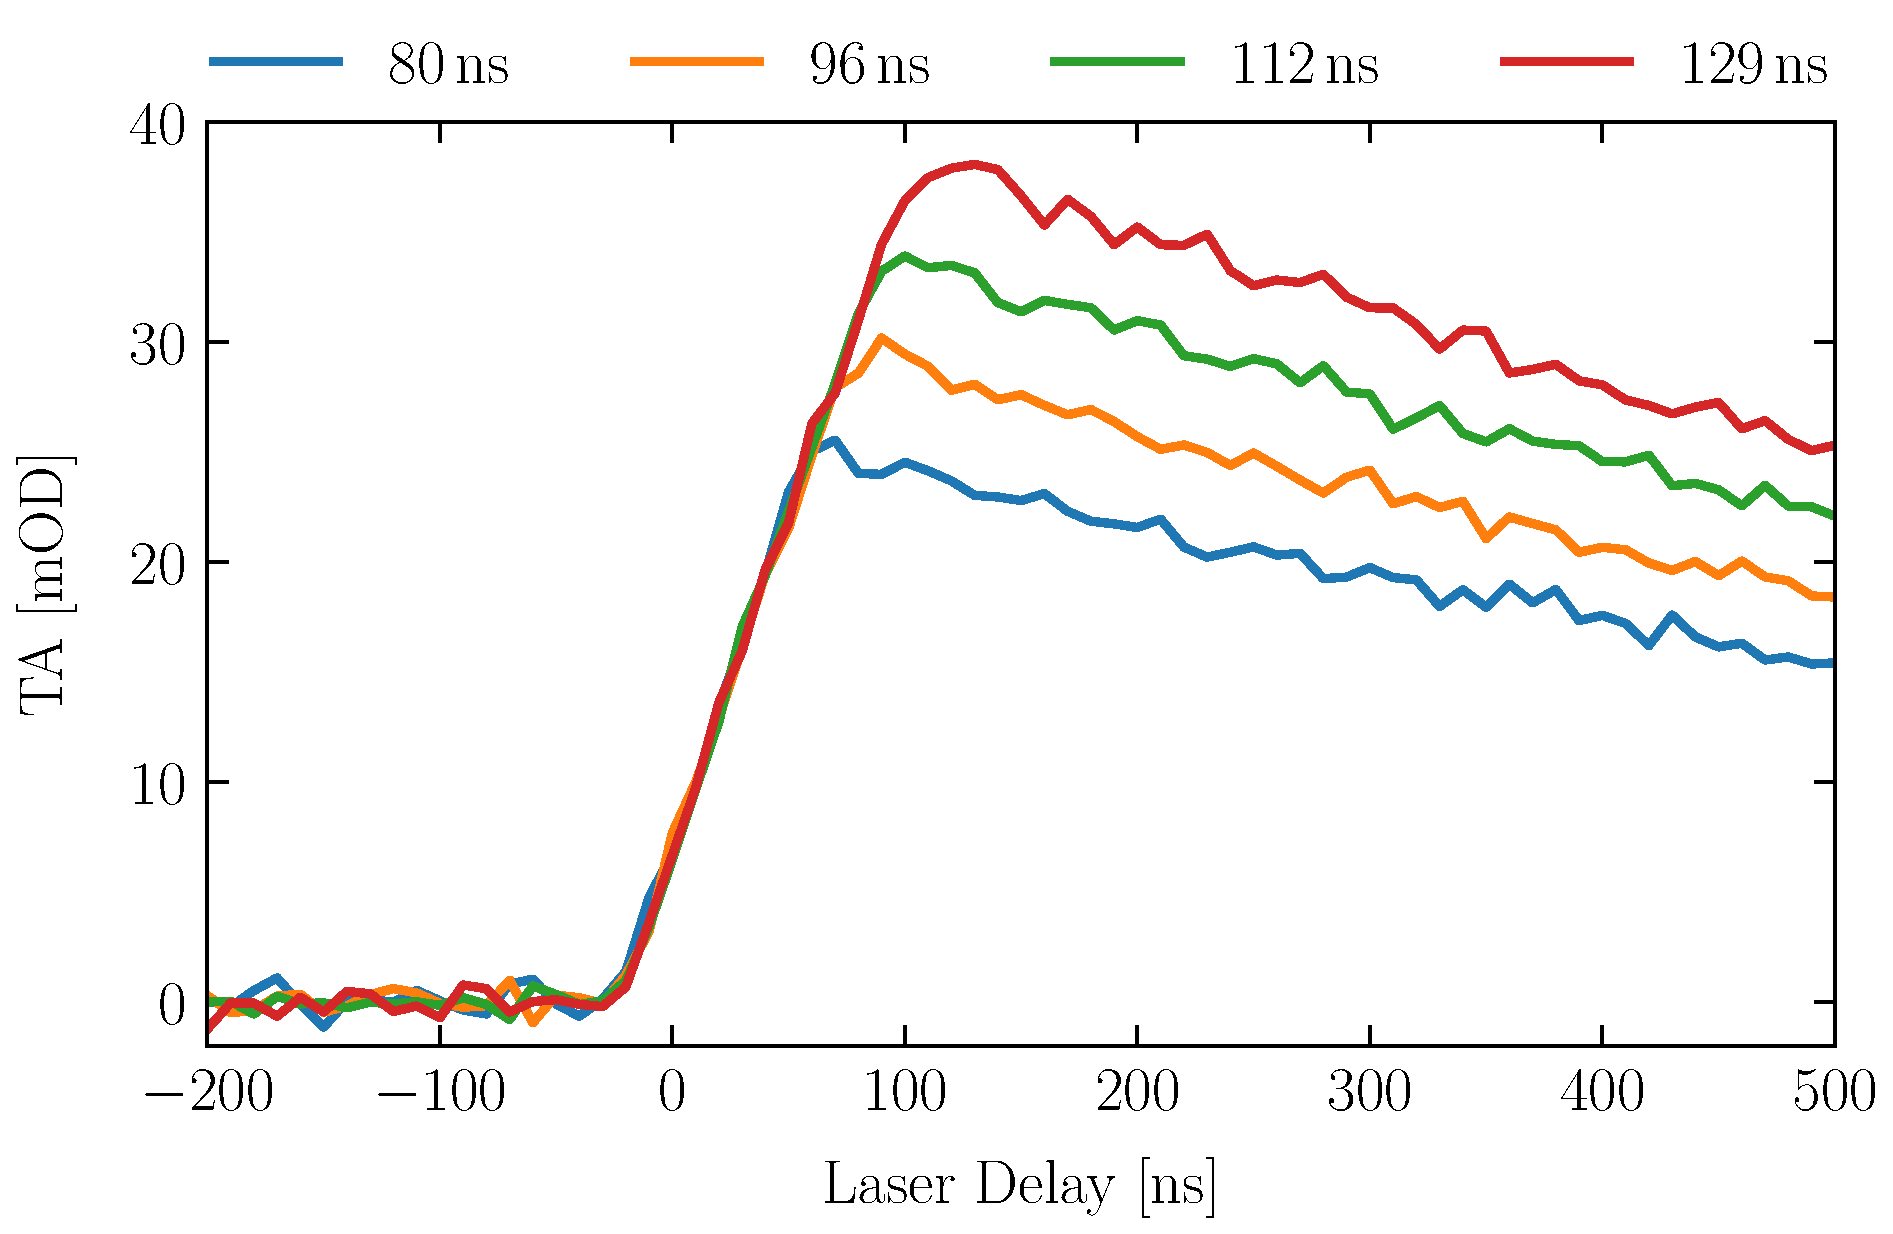
\includegraphics[width = 0.85\textwidth]{Pictures/Evaluation/42/Pump-Laser.pdf}
    \captionof{figure}{
        Transient absorption signal for different pump laser widths using ZnTPP in BN 0.8\,mM.
    }
    \label{fig:pumpLaser}
\end{center}

To investigate the influence of the pump laser width on the transient absorption (TA) signal, we measured for sample 1 [Tab. \ref{tab:lifetimeDecay}] the TA using four different pump laser widths. The TA signal is displayed in Fig. \ref{fig:pumpLaser}. In Fig. \ref{fig:pumpLaser} one can see that there is a shift in the TA maxima which correspond with the set pump laser width. This follows our expectations, since the longer pump laser should be able to exite more electrons to the triplet state. A closer look also shows that the pump laser width has no influnce on the decay rate $k_0$, i.e., the lifetime $\tau$. But to be sure a longer time interval has to be measured to determine the long time behaviour of the decay process.
\newpage

\section{Crystal structure of Zircon/Zirconium(IV)silicate (ZrSiO4)}
\label{sec:ZrSiO4}

Using the Rietveld-wizard from Jana2006 we do the peak profilingand get the profile showed in figure \ref{fig:ZrSiO4Prof} and the parameters:

\begin{align}
    a=b=6.608\,\mathrm{\AA} \quad c=5.988\,\mathrm{\AA}
\end{align}

% \begin{center}
%     \begin{sidewaysfigure}
%     \centering
%     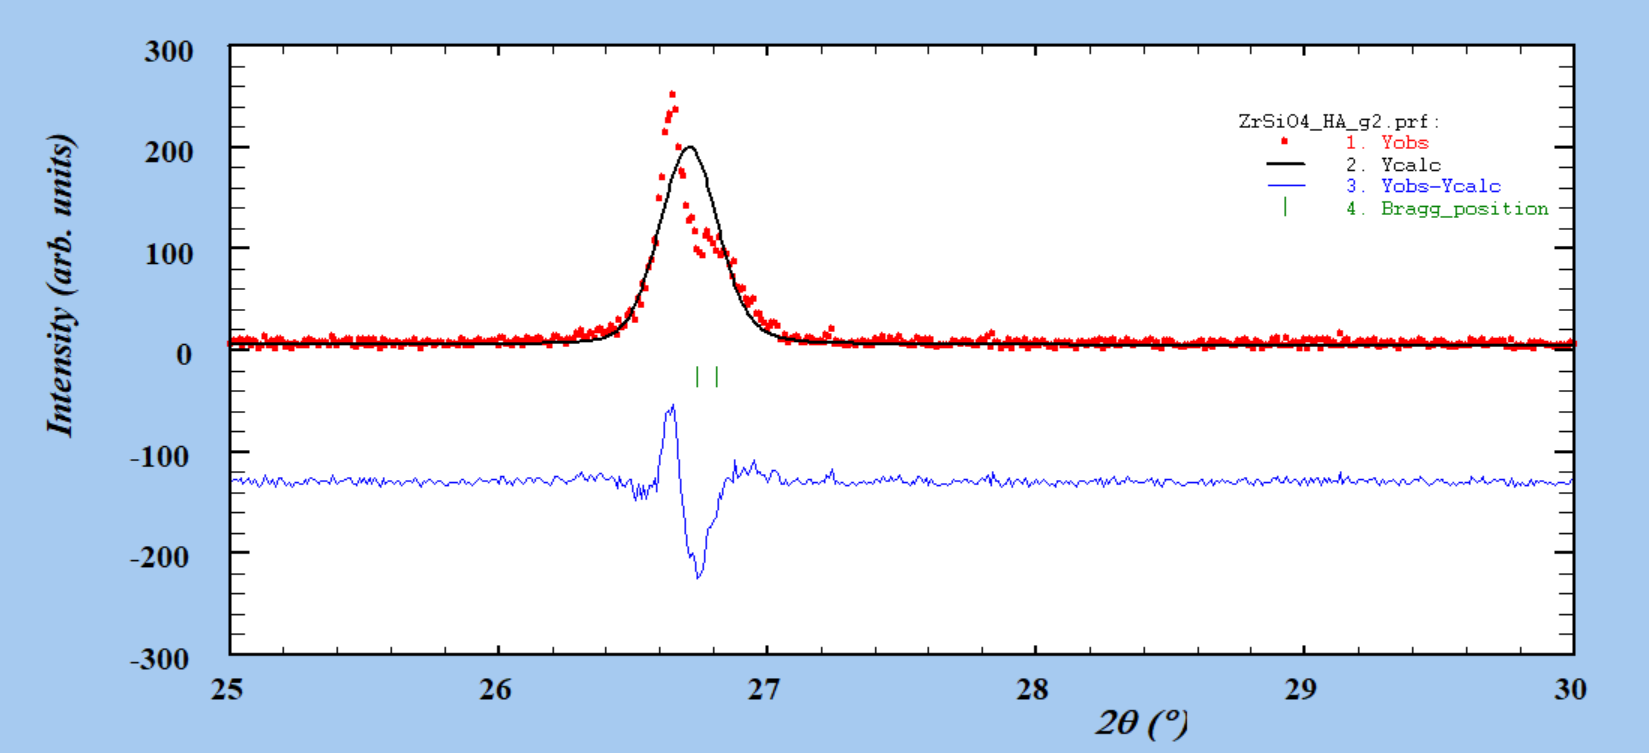
\includegraphics[width = 0.9\textheight]{Pictures/Evaluation/43/ZrSiO4DemoPeak.png}
%     \caption{
%         Due to the different distances between the $K\alpha$ lines and the two subpeaks of each peak, the profile could not be calculated exactly, but just as one pseudo-Voigt curve instead of a composition of two.
%     }
%     \label{fig:demoShitPeaks} 
%     \end{sidewaysfigure}
% \end{center}

\begin{center}
    \captionsetup{type = figure}
    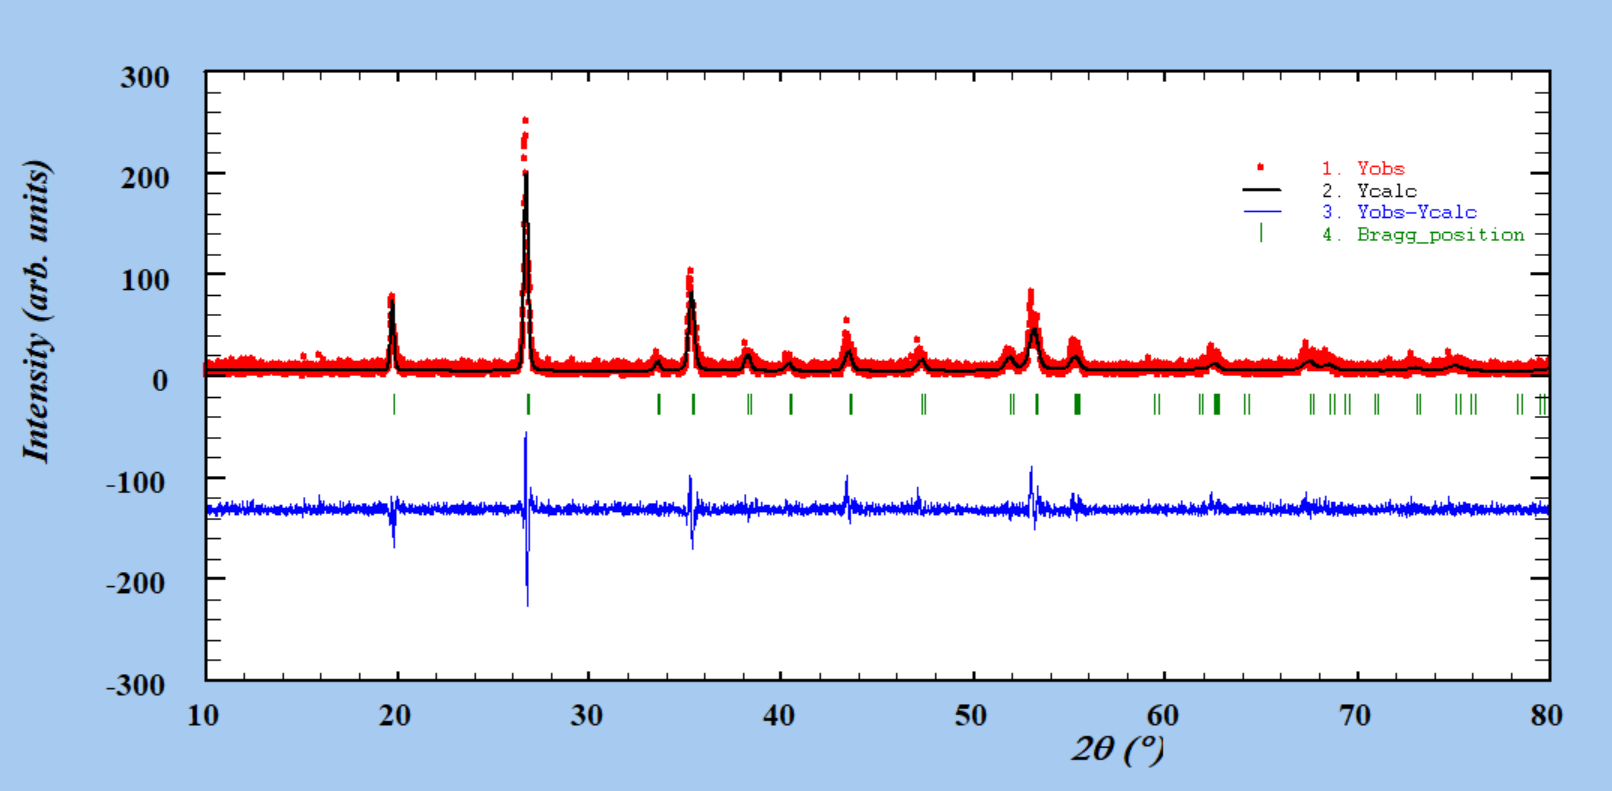
\includegraphics[width = 0.9\textwidth]{Pictures/Evaluation/43/ZrSiO4DataAll.png}
    \captionof{figure}{Resulting profile}
    \label{fig:ZrSiO4Prof}
\end{center}
Te difference plot shows some peaks,  which are due to inaccuracies.

Furthermore, the structure shown in figure \ref{fig:ZrSiO4Struct} were generated via Jana2006.


\begin{center}
    \captionsetup{type = figure}
    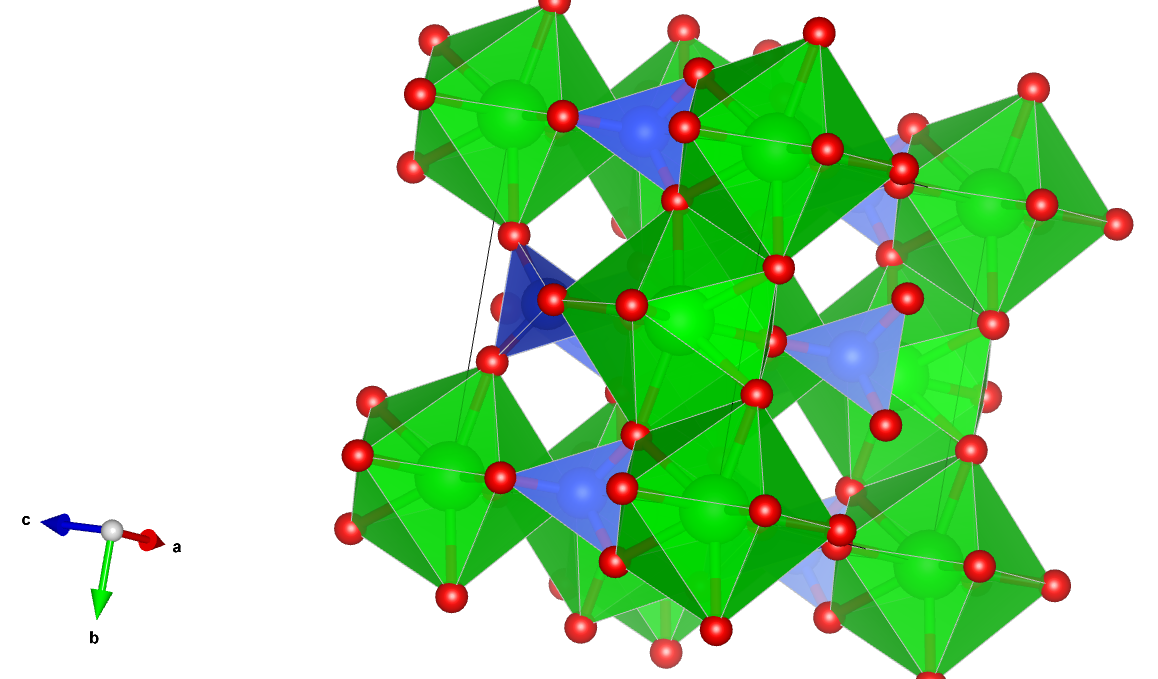
\includegraphics[width = 0.7\textwidth]{Pictures/Evaluation/43/ZrSiO4StructurePolyhedral.png}
    \captionof{figure}{
        Structure model in polyhedral style. ZrO\textsubscript{8} trigondodecahedra in green and SiO\textsubscript{4} tetrahedra in blue. 
    }
    \label{fig:ZrSiO4Struct}
\end{center}
\chapter{Methods and Material}
\label{chap:methods}

\section{Experimental Setup}
\label{sec:setup}

\section{Effect of the used Lens in the Beam Path}
\label{sec:effect}

\section{Extend Shelf Life of the Solutions}
\label{sec:lifetime}

\section{Concentration of a Polymer}
\label{sec:concentration}
\chapter{Methods and Material}
\label{chap:methods}

\section{Experimental Setup}
\label{sec:setup}

\section{Effect of the used Lens in the Beam Path}
\label{sec:effect}

\section{Extend Shelf Life of the Solutions}
\label{sec:lifetime}

\section{Concentration of a Polymer}
\label{sec:concentration}

% text

    % 3.Kapitel Protocol
    % % 3. Protocol

\chapter{Methods and Materials}
\label{chap:methods}


\section{Setup for X-ray absorption measurement}
\label{sec:SetupAbsorb}

To measure the emission spectrum of the anode, a setup as shown in Fig. \ref{fig:setupabs} is used. The X-rays are generated in an X-ray tube (RR). A monochromator, realized in a rotatable single crystal (K), 
selects a specific wavelength of the X-ray spectrum depending on the angle 2$\theta$ set. After an aperture (B), the now nearly monochromatic X-ray radiation hits the sample holder (F). Into this holder the sample
can be inserted. After the radiation passed the sample holder, the intensity of the radiation is measured by a counting tube (Z) and the data is transferred to a computer.

\begin{center}
    \captionsetup{type = figure}
    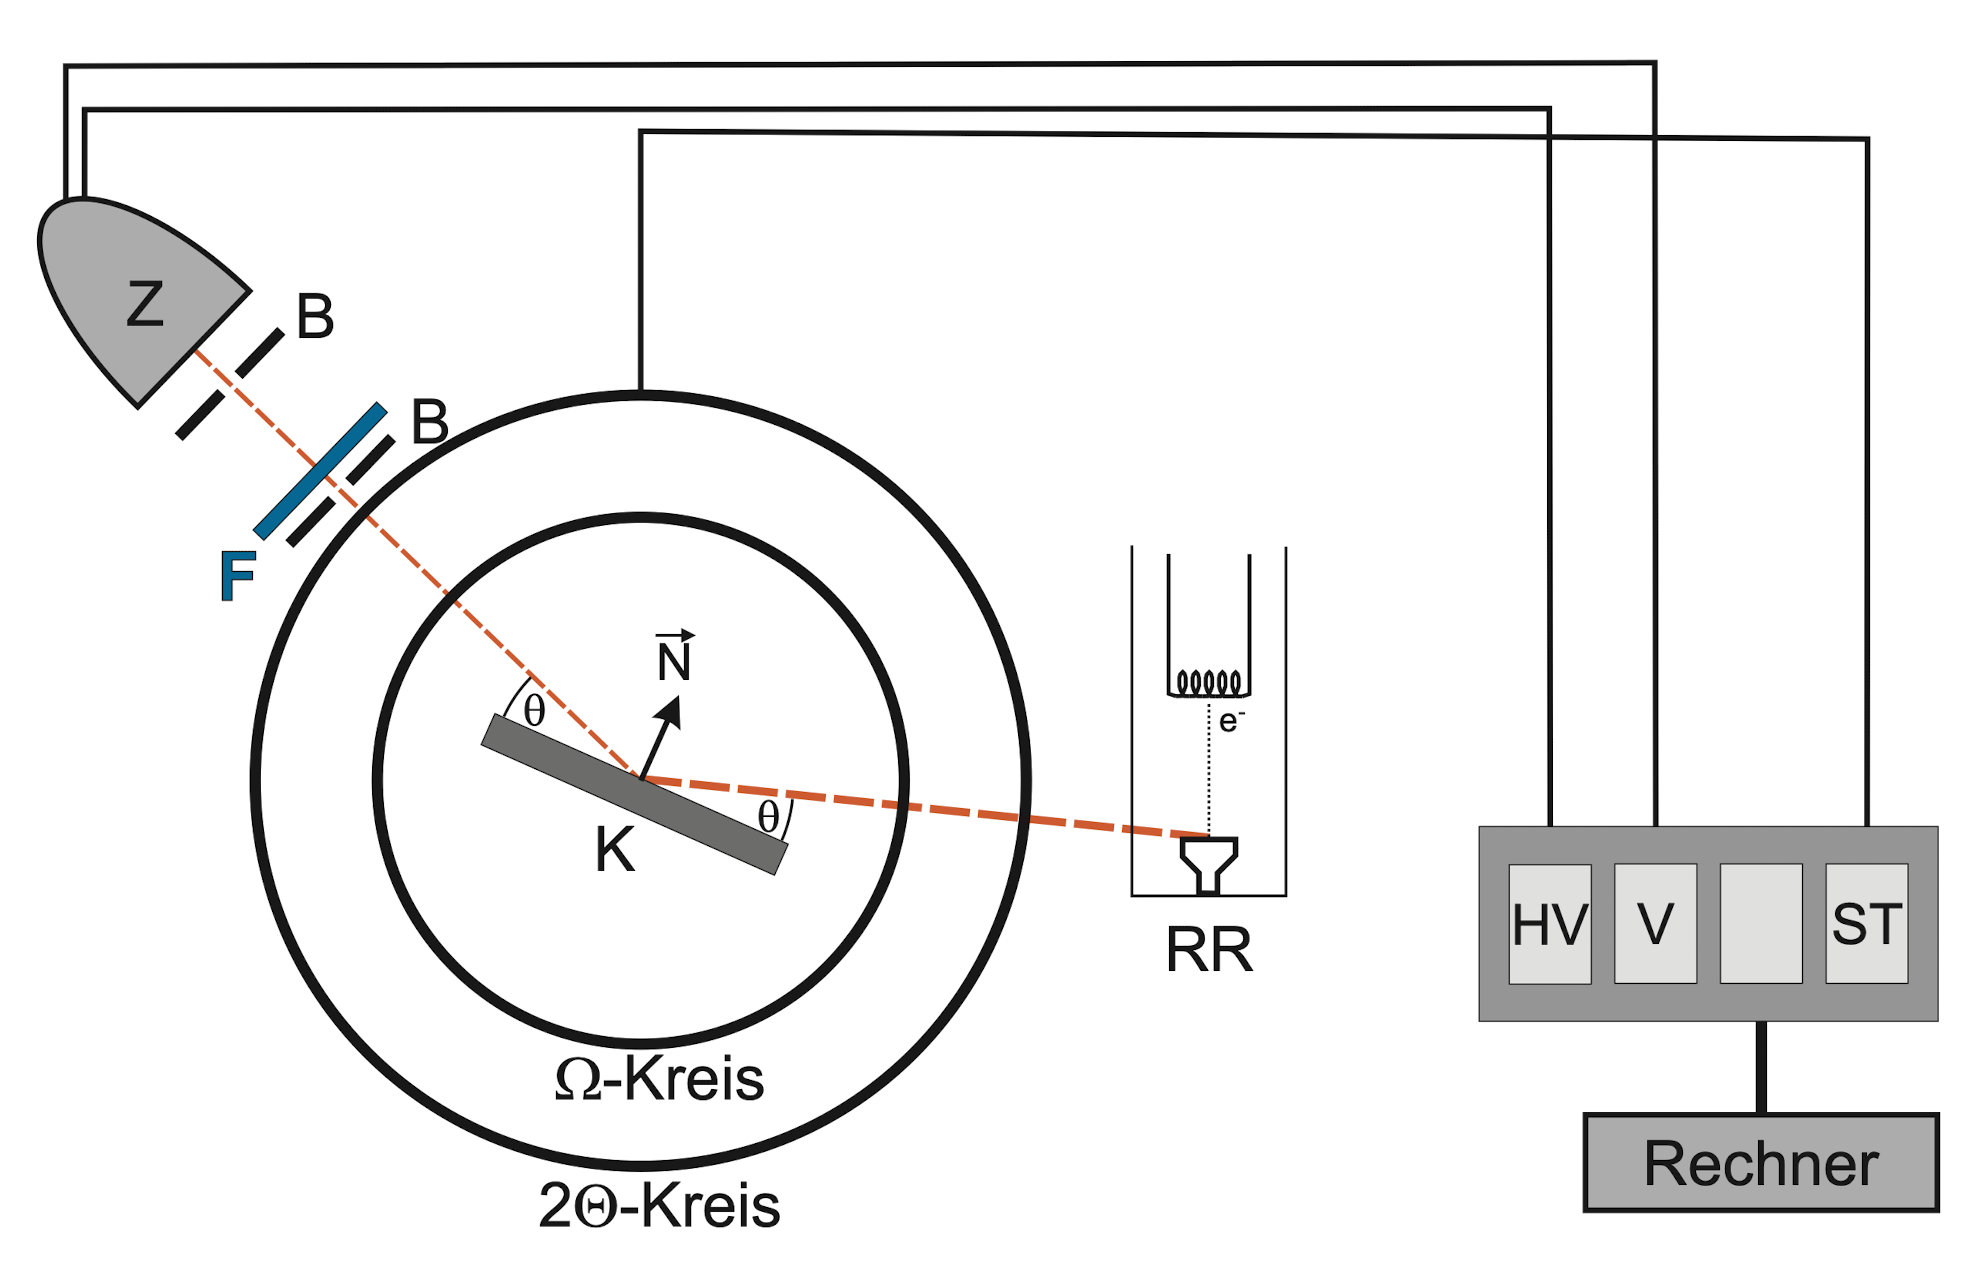
\includegraphics[width = 0.8\textwidth]{Pictures/SetupAbsorb.png}
    \captionof{figure}{
        Experimental setup of the absorption measurement
    }
    \label{fig:setupabs}
\end{center}

\newpage
\section{Setup for X-ray absorption measurement}
\label{sec:SetupDiff}

For the diffraction measurement we are using a similar setup to the setup used before. As depicted in Fig. \ref{fig:setupdiff}, the X-rays are generated in an X-ray tube (RR). Afterwards a monochromator selects one X-ray wavelength. 
The sample (S) is turned as the single crystal in the absorption setup. For each position the diffraction under 2$\theta$ is measured by a counting tube (Z) and the data is transferred to a computer.

\begin{center}
    \captionsetup{type = figure}
    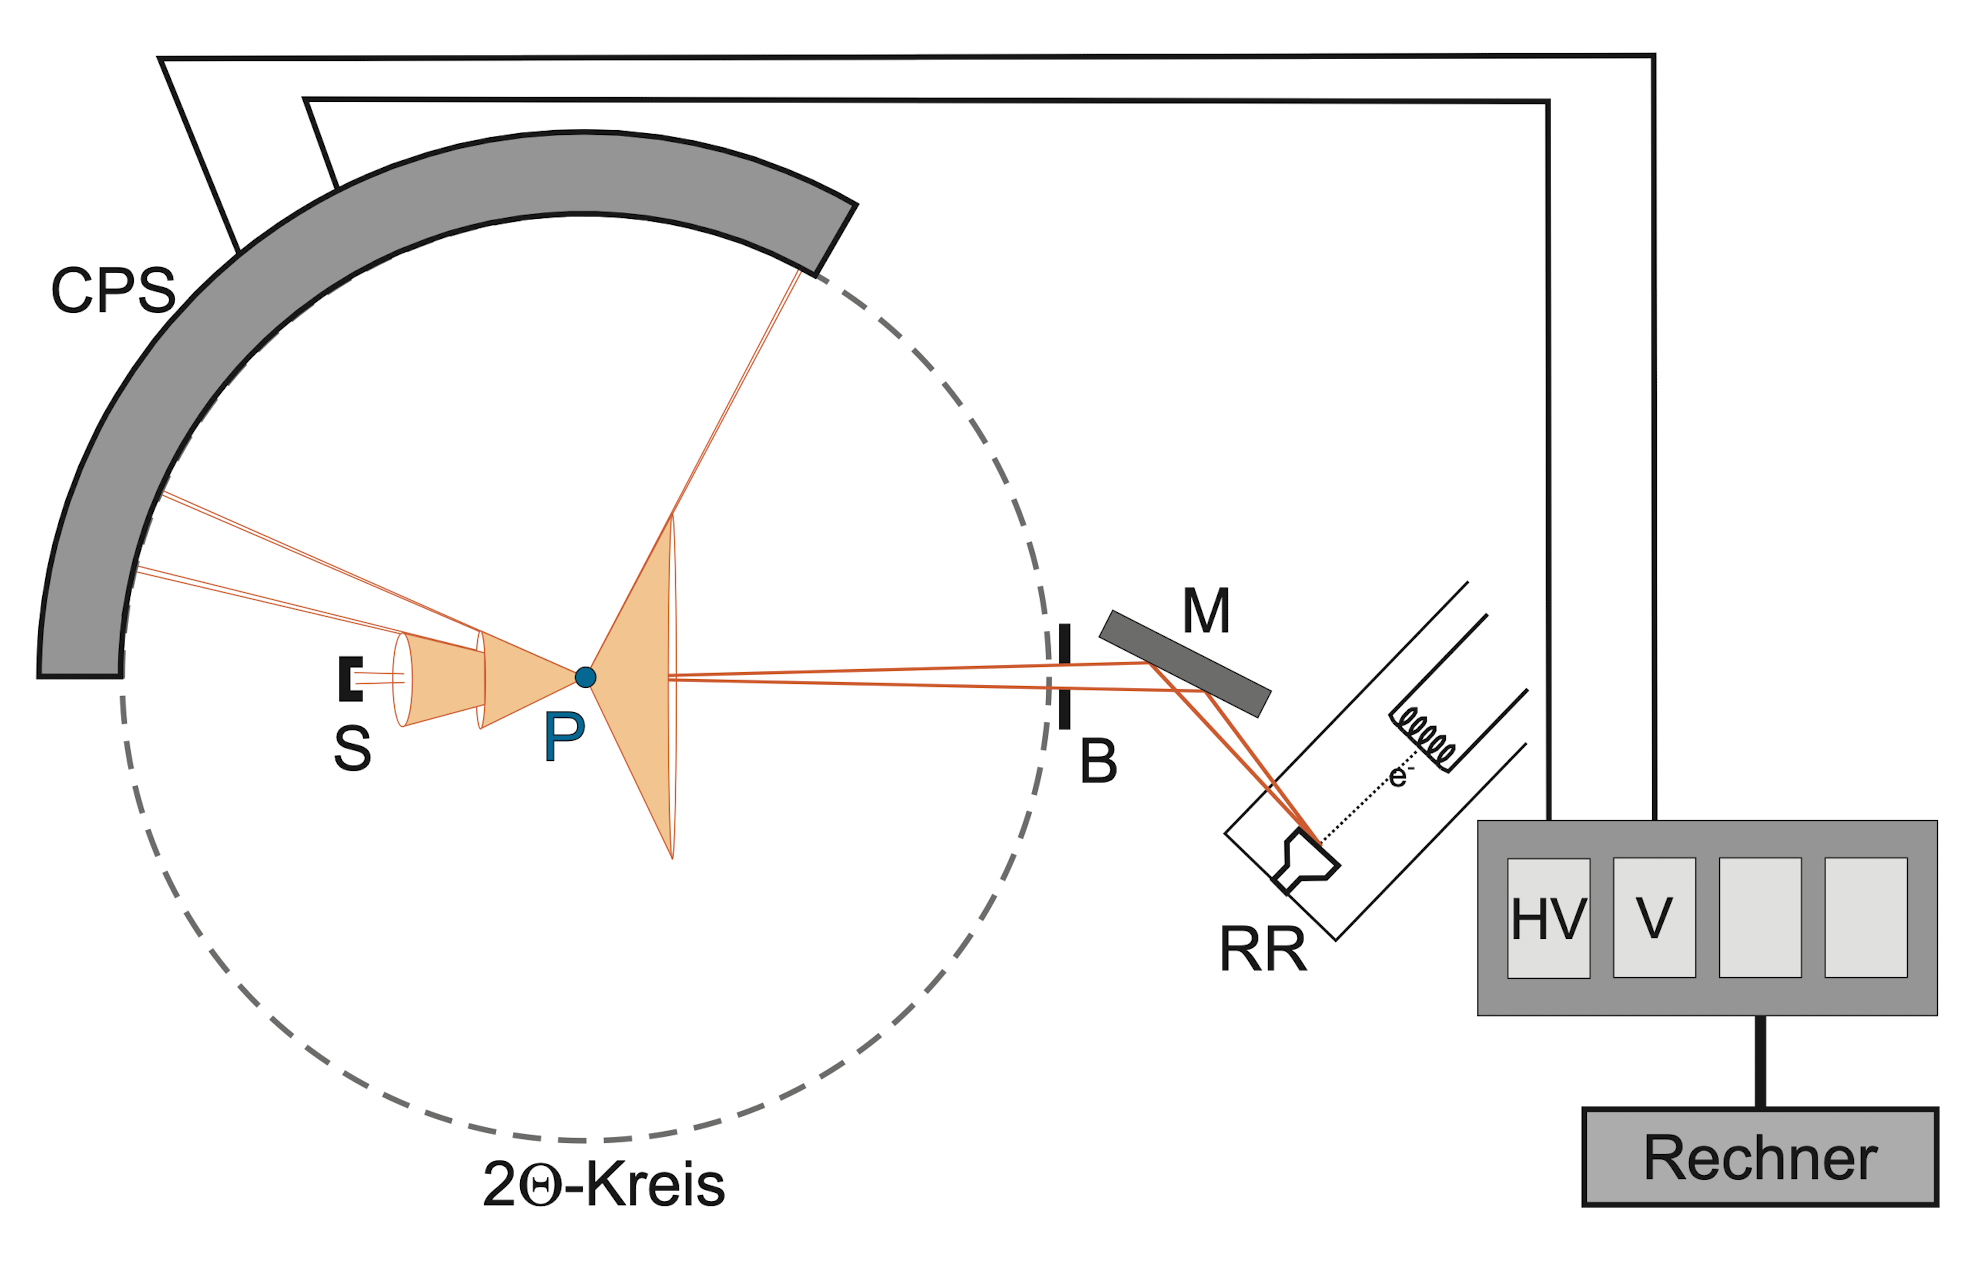
\includegraphics[width = 0.8\textwidth]{Pictures/SetupDiff.png}
    \captionof{figure}{
        Experimental setup of the diffraction measurement
    }
    \label{fig:setupdiff}
\end{center}

In the sample preparation procedure, the crystal under examination (e.g., NaCl, glucose) is finely ground using a mortar. The resulting powder should possess a fine texture, barely detectable when rubbed between the fingers. Subsequently, the powder is carefully loaded into a sample holder, paying attention to a flat surface of the powder. Finally, the sample holder is inserted into the X-ray setup and the measurement is started. The measurement process runs for
approximately one week.

    % 4.Kapitel Evaluation
    % 4. Evaluation

\chapter{Evaluation}
\label{chap:eval}

% Text

\section{Singlet and Triplet Excited States}
\label{sec:excitedStates}

\begin{center}
    \captionsetup{type = figure}
    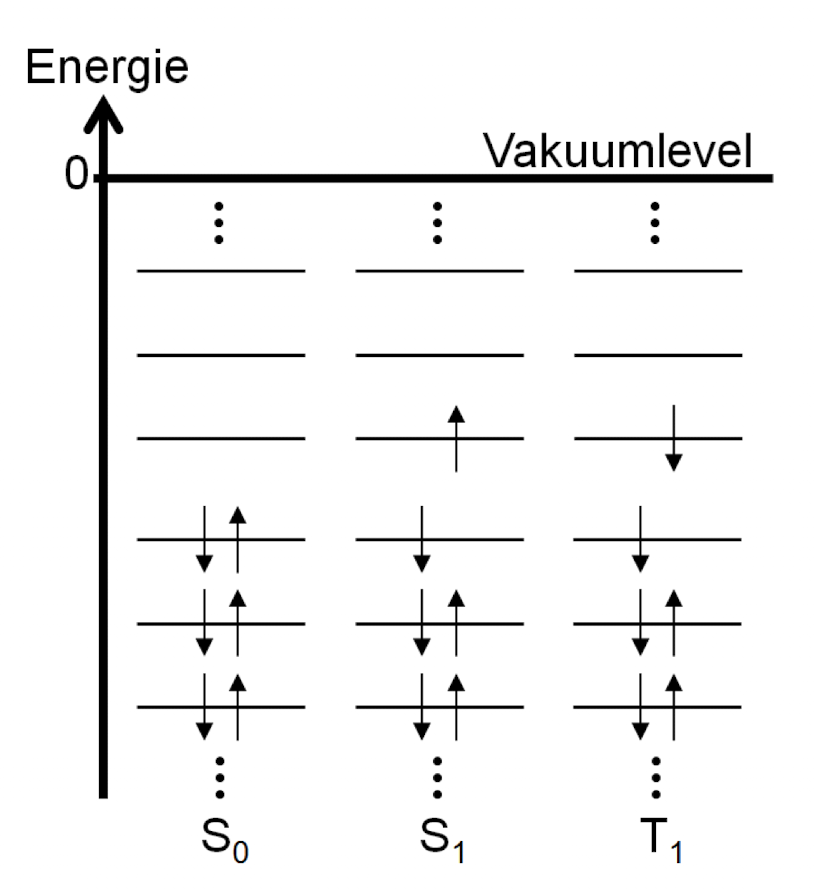
\includegraphics[width = 0.4\textwidth]{Pictures/Excited-States.png}
    \captionof{figure}{
        Orbital diagram of the dominant orbital occupations of the singlet states $S_0$ , $S_1$ and the triplet state $T_1$. \cite{Kilchert.04.2023} 
    }
    \label{fig:states}
\end{center}

In this section we want to discuss the relevant aspects of electronic processes in organic molecules. The energy levels of these systemes can be described by molecular orbitals. Molecular orbitals can be obtained through the usage of the \textbf{LCAO} method, which combines multiple atomic orbitals to a molecular orbital. A concrete occupation if these orbitals is called state, which have two specific states called \textbf{HOMO} (Highest Occupied Molecular Orbital) and \textbf{LOMO} (Lowest unOccupied Molecular Orbital). In addition to that distinction is made between singlet and triplet state with the following properties
\begin{itemize}
    \item Triplet State $T_i$: Total spin (sum of all electron spins) is $\pm 1$, 
    \item Singlet State $S_i$: Total spin is 0.
\end{itemize}
Figure \ref{fig:states} shows a simplified representation (only the largest contribution) of electronic states in molecules. 

\begin{center}
    \captionsetup{type = figure}
    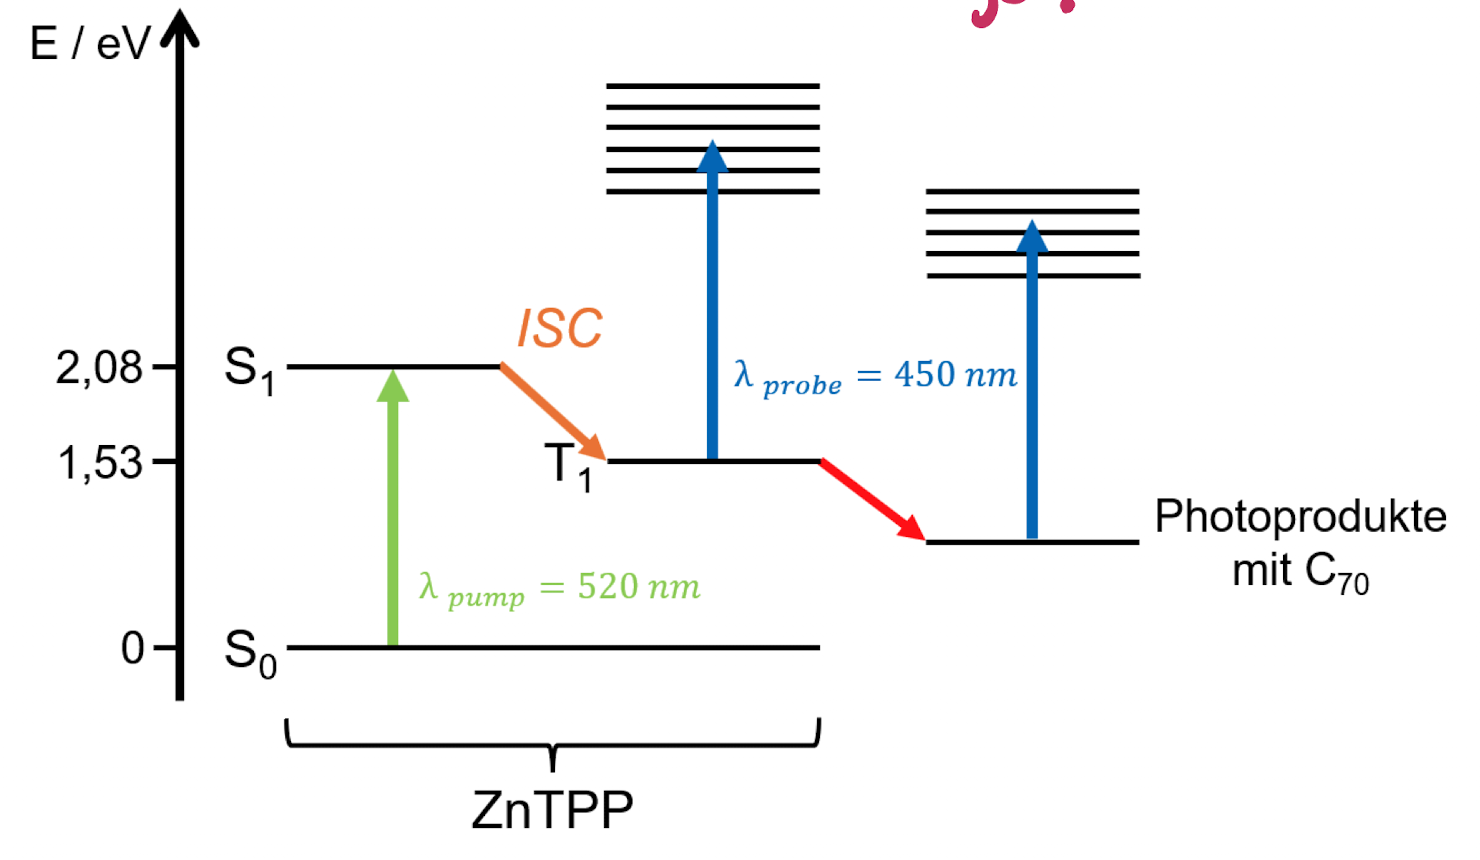
\includegraphics[width = 0.6\textwidth]{Pictures/Transition.png}
    \captionof{figure}{
        Jablonski scheme of the system of this experiment (ZnTPP and ZnTPP with fullerene $\mathrm{C}_{70}$). \cite{Kilchert.04.2023} 
    }
    \label{fig:transition}
\end{center}
To excite a system into from the ground state to the singlet state the system has to absorbe a photon with the energy corresponding to the transition, which leads to an absorption pattern the refelcts the structure of the energy levels of an atom. After absorption the electron relaxes back into the ground state (\textit{Kasha's Rule}). The transition can be radiative or non-radiative, but it is also possible to perform a transfer to a triplet state if the energy gap is small enough and one spin is flipped, which results in a sufficiently large spin-orbit coupling. The transition between singlet to triplet states is called Inter System Crossing (ISC). The jablonski scheme of this transition process for the relevant molecule of this experiment (ZnTPP and ZnTPP with fullerene $\mathrm{C}_{70}$) is shown in Figure \ref{fig:transition}. 
\bigskip

The radiative transition of an electron from the singlet state to the ground state is called \textbf{Flourescence} and from a triplet state to the ground state \textbf{Phosphorescence}. Both mentioned transitions are examples for \textit{radiative decays} with the emission of a photon. In case of ISC it is a \textit{non-radiative decay}, since the energy of the excited singlet state gets disspated due to ISC. The lifetime $\tau$ of the excited state will be given by the expression
\begin{gather}
    \tau = \frac{1}{k_\mathrm{r} + k_\mathrm{nr}},
\end{gather}
with the $k_\mathrm{r}$ and $k_\mathrm{nr}$ as the decay rates of the radiative and non-radiative decay. The determination is achieved by a pump-probe experiment, which will be discussed in Chapter \ref{sec:transient}. \cite{Kilchert.04.2023}
Scince the process of ISC is non-radiative one can not directly measure ISC, but if the energy level aif the singlet state is known and the decay rate of the triplet state will be measured, it is possible to indirectly measure the energy loss of ISC.
\newpage
\section{Transient Absorption Spectroscopy}
\label{sec:transient}

In this experiment different treatments were investigated in terms of lifetime $\tau$ of the solution itself. At the beginning we expect from theory that the decay of the concentration of the triplet state $C_\mathrm{T}(t)$ is exponential and given by the relation
\begin{gather}
    C_\mathrm{T}(t) = C_\mathrm{T}(0) e^{-k_0 t} + C_\mathrm{T}^\mathrm{Off}~,
    \label{eq:fitExp}
\end{gather}
with the initial concentration $C_\mathrm{T}$ and the decay rate $k_0$. Also, an offset concentration $C_\mathrm{T}^\mathrm{Off}$ was added to encounter any offset cuased by e.g. measuring methods. Since the transient absorption (TA) is porportional to $C_\mathrm{T}(t)$, we can fit the same exponential decay for the transient absorption as well. The full set of fitted treatments and results of the exponential fit can be found in Tab. \ref{tab:lifetimeDecay}. The lifetime $\tau$ was calculated with the relation $\tau = 1/k$. The exponential fits itself are displayed in Fig. \ref{fig:lifetimeDecay}\,.
\begin{center}
    \captionsetup{type = table}
    \begin{tabular}{| c | l | c c |}
        \hline
        No & Treatment             & $k_0$/ms$^{-1}$            & $\tau$/ns   \\\hline
        1  & ZnTPP in BN 0.8\,mM   & 1089 $\pm$ 4               & 919 $\pm$ 3 \\
        2  & ZnTPP in BN 0.6\,mM   & 1077 $\pm$ 5               & 929 $\pm$ 4 \\
        3  & ZnTPP in BN 0.4\,mM   & 1069 $\pm$ 5               & 936 $\pm$ 4 \\
        4  & ZnTPP in BN 0.2\,mM   & 1057 $\pm$ 8               & 946 $\pm$ 7 \\\hline
        8  & ZnTPP in Tol 0.8\,mM  & 1891 $\pm$ 3               & 529 $\pm$ 1 \\\hline
        12 & ZnOEP in BN 0.8\,mM   & 2681 $\pm$ 5               & 373 $\pm$ 1 \\\hline
        \multicolumn{4}{c}{}\\\hline
        No & Treatment             & $k_\mathrm{app}$/ms$^{-1}$ & $\tau$/ns   \\\hline
        5  & ZnTPP:C70 in BN 1:0.1 & 1254 $\pm$ 5               & 798 $\pm$ 3 \\
        6  & ZnTPP:C70 in BN 1:0.2 & 1385 $\pm$ 6               & 722 $\pm$ 3 \\
        7  & ZnTPP:C70 in BN 1:0.3 & 1436 $\pm$ 6               & 697 $\pm$ 3 \\\hline
    \end{tabular}
    \captionof{table}{
        Calculated decay rates $k_0$ and $k_\mathrm{app}$ and lifetimes $\tau$ ($\tau = 1/k$) for different types of treatments.
    }
    \label{tab:lifetimeDecay}
\end{center}

\subsection{Influence of Concentration}
\label{sub:concentration}

First, we want to investigate the influence of concentration on the deacy rate $k_0$, i.e., the lifetime $\tau$. For that we take a closer look at sample number $1-4$ [Tab. \ref{tab:lifetimeDecay}]. In Fig. \ref{fig:lifetimeDecay}\,(a) it is clear that higher maxima correspond with to higher concentration of ZnTPP, which aligns with our expectation that higher concentration leads to a greater amount of absorption. The lifetime $\tau$ on the other hand increases with the reduction of concentration, which follows the expectation from the theory. The kinetics iof the decay of the triplet state are described by the equation
\begin{gather}
    \frac{\mathrm{d}}{\mathrm{d}t} C_\mathrm{T} = -k_1 C_\mathrm{T}(t) - k_2(C_\mathrm{T}(t))^2 - k_3C_\mathrm{T}(t)C_\mathrm{G}(t)~,
    \label{eq:kineticsTriplet}
\end{gather}
where $C_\mathrm{G}(t)$ is the concentration of the ground state and $k_1, k_2, k_3$ are decay rates. In further calculation the assumption $C_\mathrm{T}(t) \ll C_\mathrm{G}(t)$ will be made, which leads to the discussed exponential decay [Eq. (\ref{eq:fitExp})]. But, this assumption gets less valid for an increasing population of triplet states, to the point at which one has to take the terms with $C_\mathrm{T}(t)$ into account. This results in higher decay rates $k_0$ and shorter lifetimes $\tau$ of the triplet states. The same behaviour can be identife to the cases of higher concentration of ZnTPP in BN and explains the kinetics of the decay process.

\subsection{Influence of Fullerene \boldmath{$\mathrm{C}_{70}$}}
\label{sub:fullerene}

In the next paragraph the impact of the fullerene $\mathrm{C}_{70}$ on the lifetime $\tau$ will be addressed. We consider for this analysis sample 1 (base solution) and $5-7$ [Tab. \ref{tab:lifetimeDecay}]. In Fig. \ref{fig:lifetimeDecay}\,(b) one can see that the decreases the higher the concentration of the fullerene $C_\mathrm{q}$ gets, introducing a quenching process. This result was expected, because in theory the decay rate $k_0$ gets expanded as
\begin{gather}
    k_0 \longrightarrow k_\mathrm{app} = k_0 + k_\mathrm{q}C_\mathrm{q}~,
    \label{eq:decayExpand}
\end{gather}
with the new decay rate $k_\mathrm{app}$ and the reaction rate of quenching process $k_\mathrm{q}$. The expansion of the decay rate $k_0$ leads to higher decay rates $k_\mathrm{app}$ ($k_\mathrm{q} > 0$), which leads to shorter lifetimes $\tau$. To determine the quenchning reaction rate $k_\mathrm{q}$, we take the calculated decay rates $k_\mathrm{app}$ and fit them against the concentration $C_\mathrm{q}$ [Eq. \ref{eq:decayExpand}]. For the decay rate $k_0$ the decay rate of the base solution (sample 1) will be used. From the slope of the linear fit one can calculate the quenchning reaction rate $k_\mathrm{q}$. The linear fit can be seen in Fig. \ref{fig:concentration}. 

\begin{center}
    \captionsetup{type = figure}
    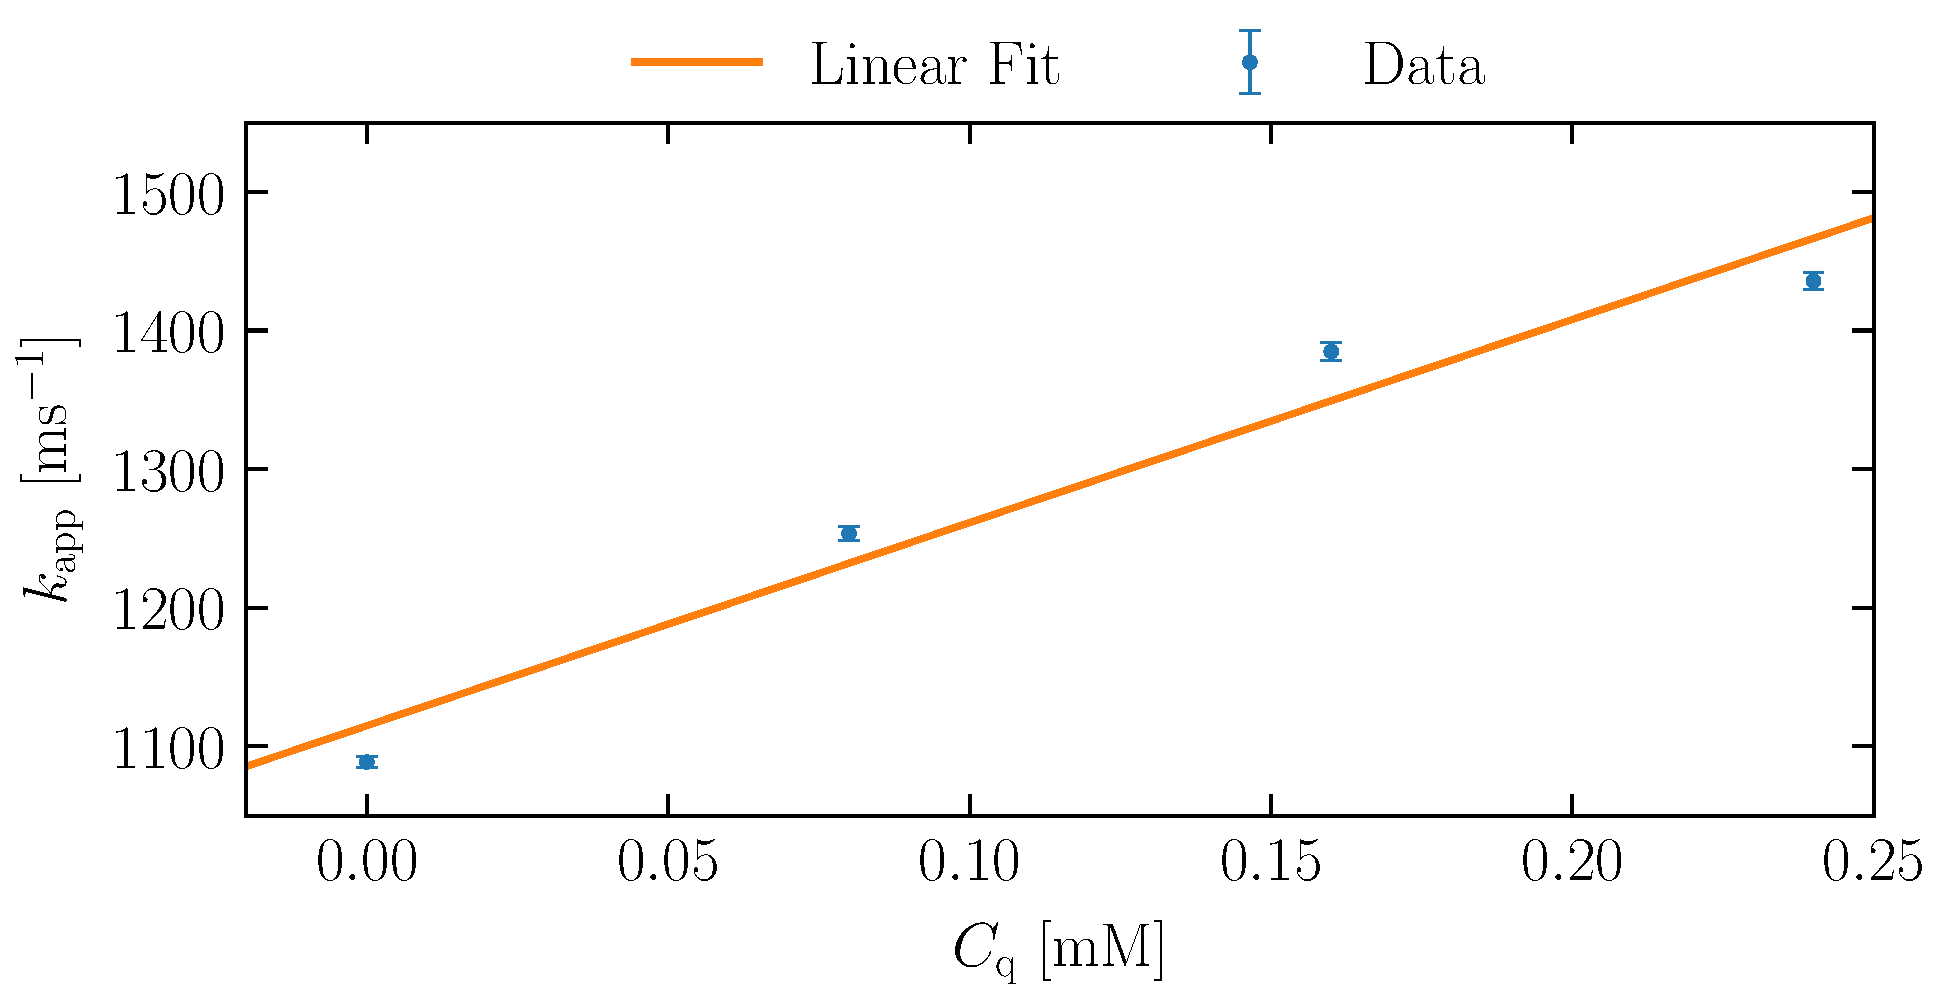
\includegraphics[width = 0.85\textwidth]{Pictures/Evaluation/42/Concentration.pdf}
    \captionof{figure}{
        Linear fit of decay rate $k_\mathrm{app}$ for different fullerene concentration $C_\mathrm{q}$. 
    }
    \label{fig:concentration}
\end{center}

The calculation yields
\begin{gather*}
    \boxed{k_\mathrm{q} = (1.5 \pm 0.2) \times 10^9\,\mathrm{sM^{-1}}}~, %1465.49 229.41 ms-1/mM
\end{gather*}
which does not align with the result of Ito et al.\cite{Nojiri.1998}, who determined $k_\mathrm{q} = 4.7 \times 10^9\,\mathrm{sM^{-1}}$, but is in the right order of magnitude.

\subsection{Influence of the Solvent}
\label{sub:difference}

In this paragraph the influence of Solvent on the transient absorption (TA) signal and the lifetime $\tau$ will be dicussed. 
\bigskip

First, we look at the variation of ZnTPP with BN and Tol for the concentration 0.8\,mM (sample 1 and 8 [Tab. \ref{tab:lifetimeDecay}]). In Fig. \ref{fig:lifetimeDecay}\,(c) we can observe the nearly same maximum value for both solutions but different lifetimes $\tau$, which are calculated in Tab. \ref{tab:lifetimeDecay}. This aligns with the UV-VIS spectroscopy from Chapter \ref{sec:uv-vis}, because the polarity of BN makes it easier to induce more charges into the delocalized $\pi$-electron system. So, it is possible to observe a redshift and an increase of lifetime $\tau$. 
\bigskip

Next, we vary the zinc complexes of the solution from ZnTPP to ZnOEP, but we keep BN as second solvent of the solution with concentration 0.8\,mM (sample 1 and 12 [Tab. \ref{tab:lifetimeDecay}]). The transient absorption signal can be found in Fig. \ref{fig:lifetimeDecay}\,(d) with the corresponding decay rates $k$ and lifetimes $\tau $ in Tab. \ref{tab:lifetimeDecay}. It is clearly visible that the maximum of the TA signal is for both zinc complexes the same but the lifetime $\tau$ for is much shorter for ZnOEP. The value of the TA maximum corresponds with the maximum concentration of the triplet state and is therefor correlated to the absorption of the pump laser light. Looking at the UV-VIS of ZnTPP and ZnOEP [Fig. \ref{fig:uv-visZinc}] one can conclude that the absorbance for ZnTPP and ZnOEP does not differ from each other, which explains teh same maximum value for the TA signal. The longer lifetime $\tau$ of ZnTPP can also be linked to the redshift compared to ZnOEP. Due to the four additional phenyl groups in ZnTPP, the conjugated electron system is bigger than in ZnOEP. So, a lower energy is needed to exite the electrons of ZnTPP.
\bigskip

Finally, we want to discuss the variation of the solution itself. For that, we take a look at sample 1 (ZnTPP in BN 0.8\,mM) and 9 (P3HT in Tol 1.5\,mM). In Fig. \ref{fig:difference} it is visible that P3HT has a smaller maximum compared to ZnTPP. From the previous lifetime analysis one can assume trivial that the lifetime of P3HT is shorter compared to the lifetime of ZnTPP. Comparing the UV-VIS of P3HT from Ref. \citenum{Rahimi2014} to the evaluation from ZnTPP from Chapter \ref{sec:uv-vis} the observed redshift is also present for P3HT as well as the smaller absorbance compared to ZnTPP. The underlying process relates to the P3HT aggregates, which can consist of crystalline regions, amorphous domains or a combination of both. Amorphous chain sequences lead to structural defects, grain boundaries and coiled-like chain conformations that can reduce intra-chain order. Therefore, UV-VIS absorption signatures are broadened and blue shifted towards higher energies \cite{Rahimi2014}, which results in the observed (TA) signal.

\begin{center}
    \captionsetup{type = figure}
    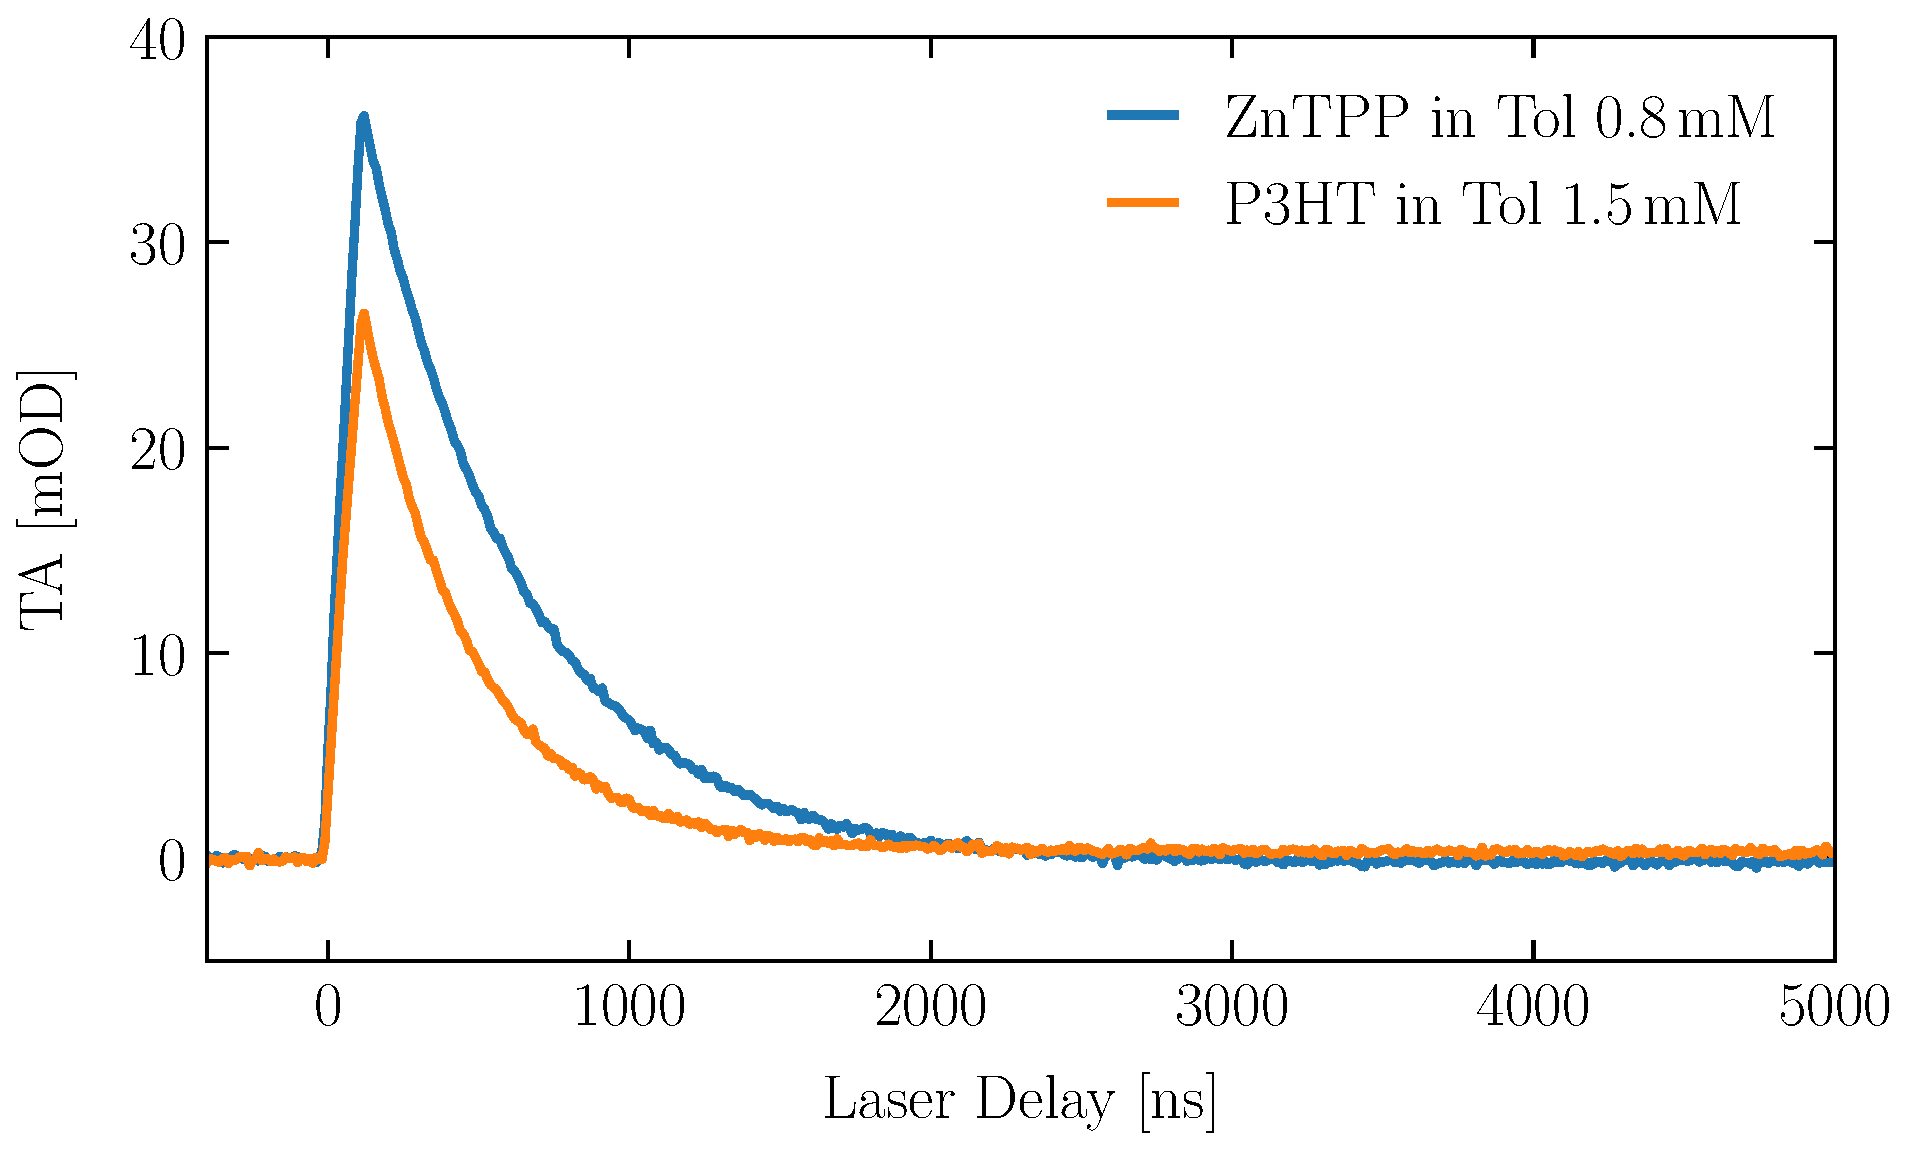
\includegraphics[width = 0.85\textwidth]{Pictures/Evaluation/42/Difference.pdf}
    \captionof{figure}{
        Transient absorption signal using different treatments with ZnTPP and P3HT 
    }
    \label{fig:difference}
\end{center}

\begin{center}
    \begin{sidewaysfigure}
    \centering
    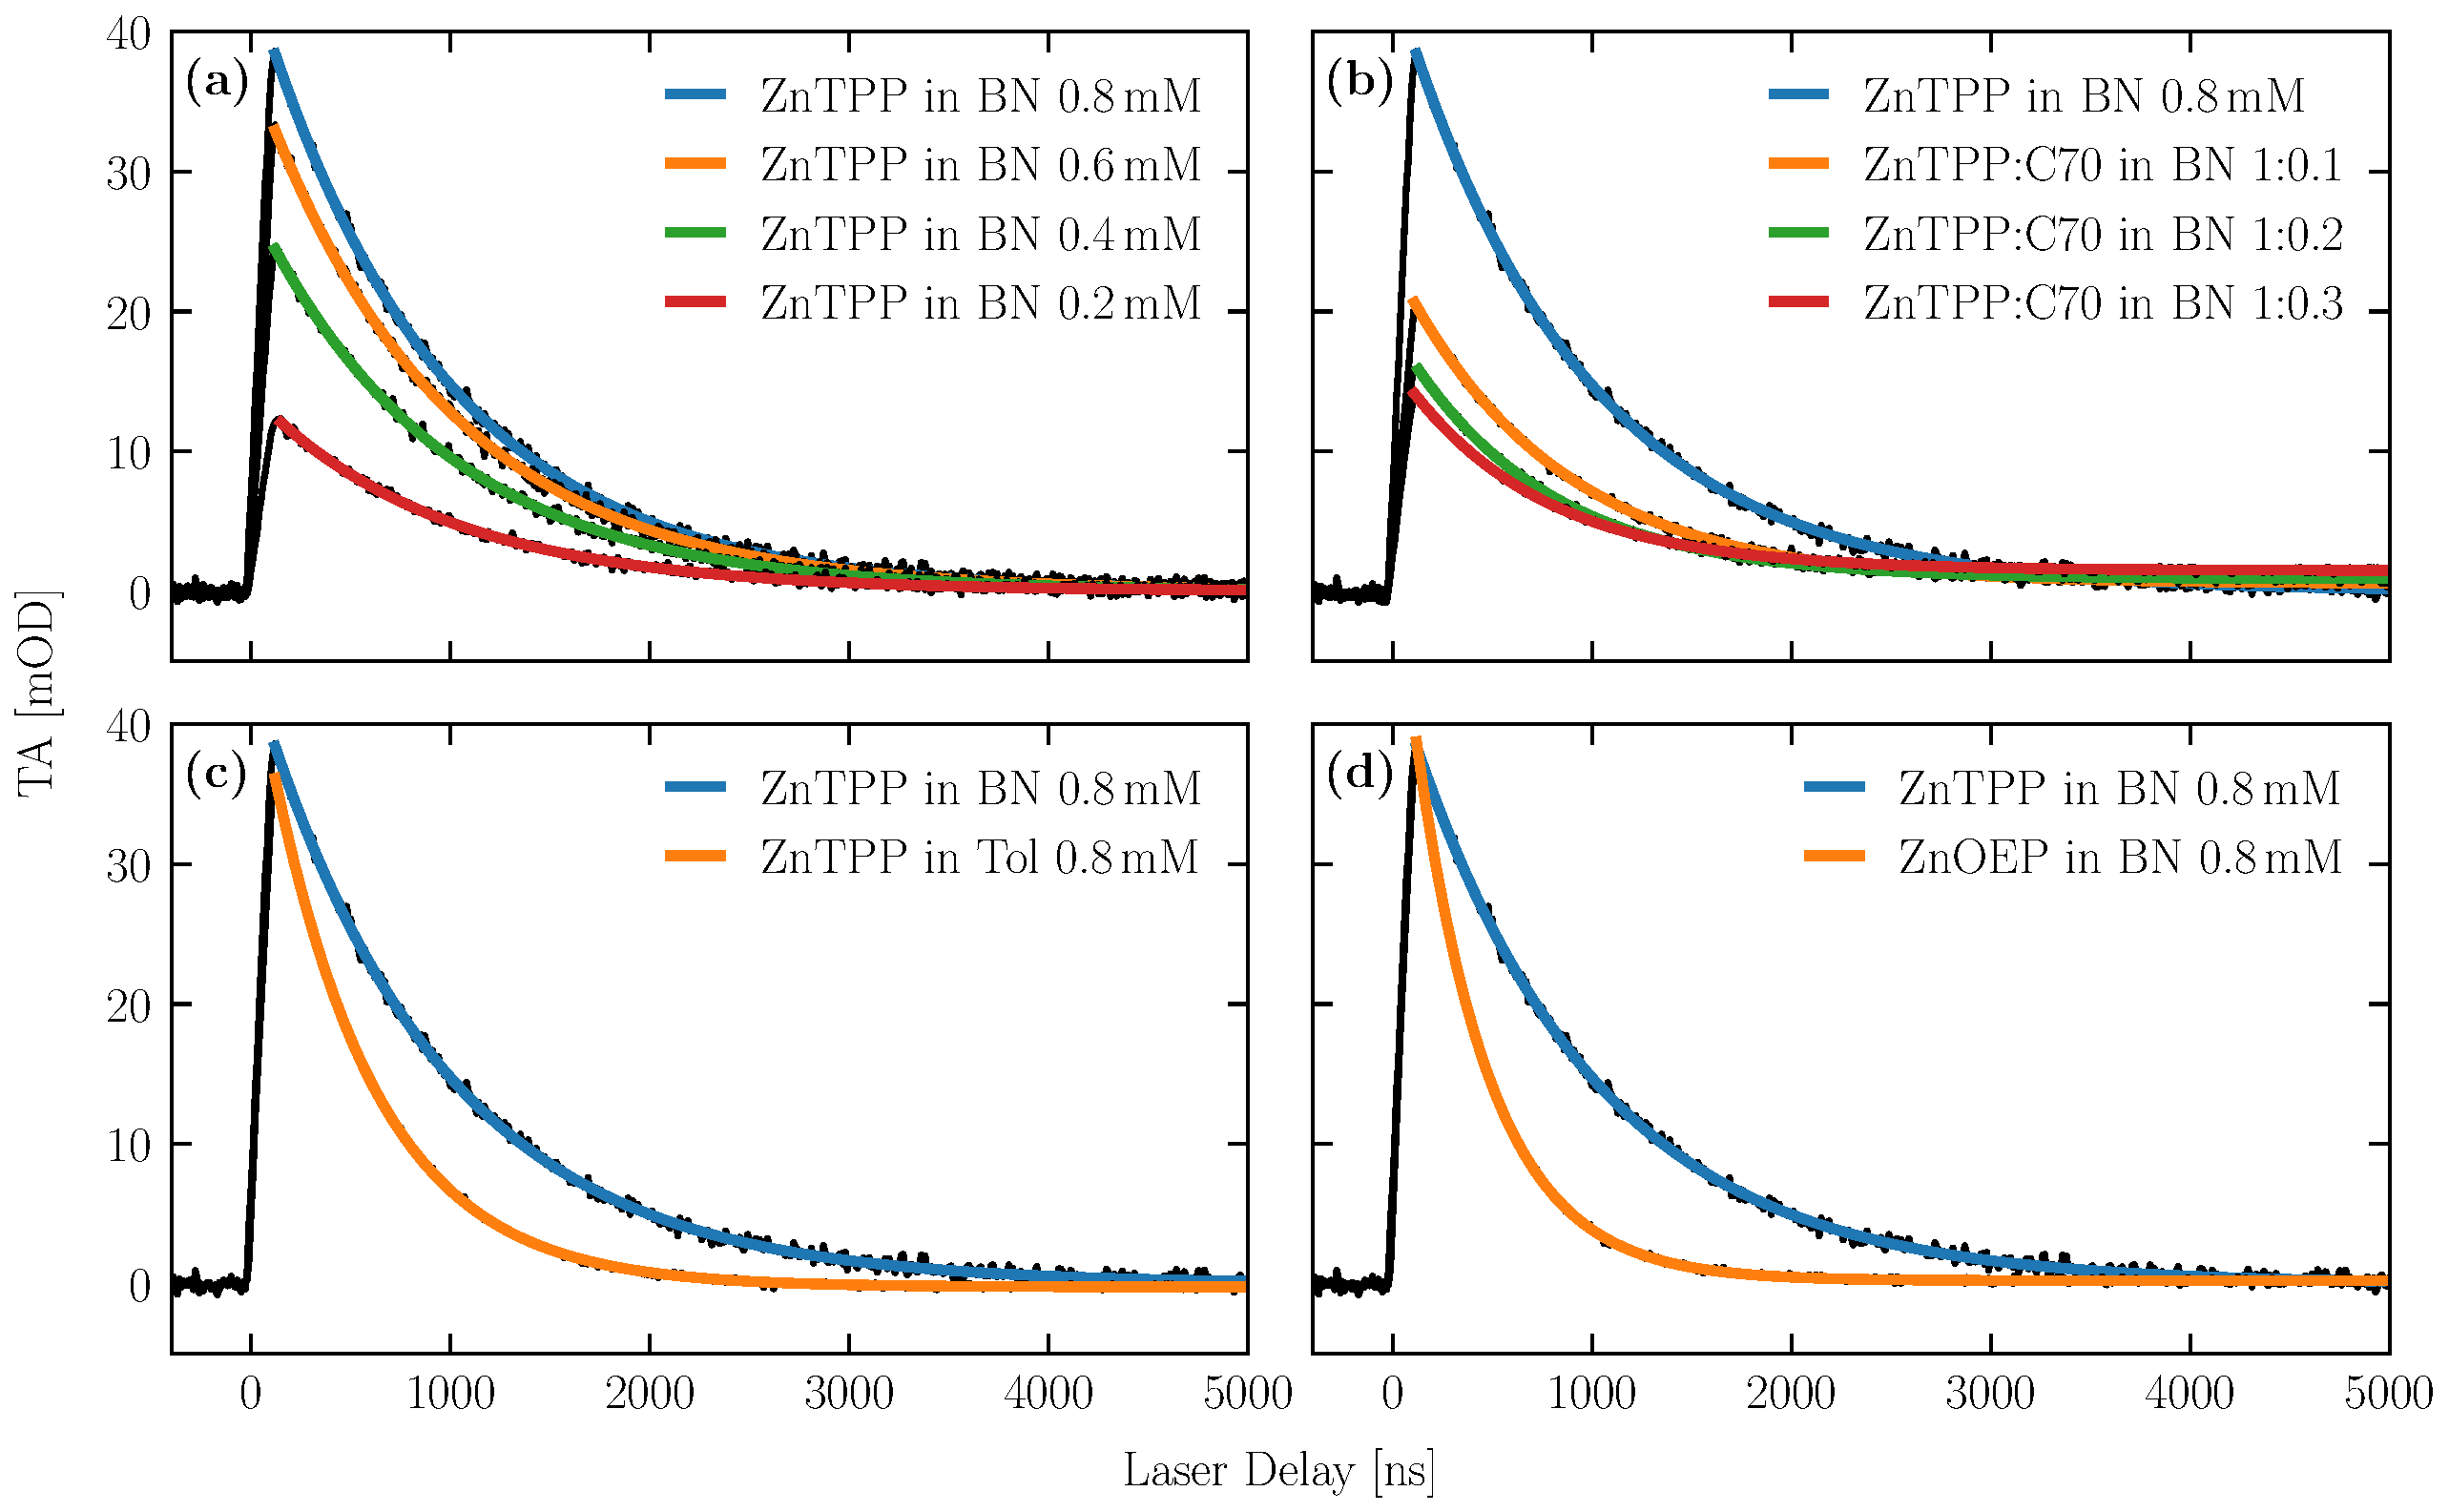
\includegraphics[width = 0.9\textheight]{Pictures/Evaluation/42/Lifetime.pdf}
    \caption{
        Comparison between data of the transient absorption of different treatments with the exponential fits colored for each treatment: (a) Different concentration of ZnTPP in BN, (b) Different dullutions of C$_{70}$ in ZnTPP in BN 0.8\,mnM, (c) Different Solvents (BN, Tol) with ZnTPP and a concentration of 0.8\,mM and (d) Different Solvents (ZnTPP, ZnOEP) with BN and a concentration of 0.8\,mM.
    }
    \label{fig:lifetimeDecay}
    \end{sidewaysfigure}
\end{center}
\newpage

\subsection{Influence of the Pump Laser Width}
\label{sub:pumpLaser}

\begin{center}
    \captionsetup{type = figure}
    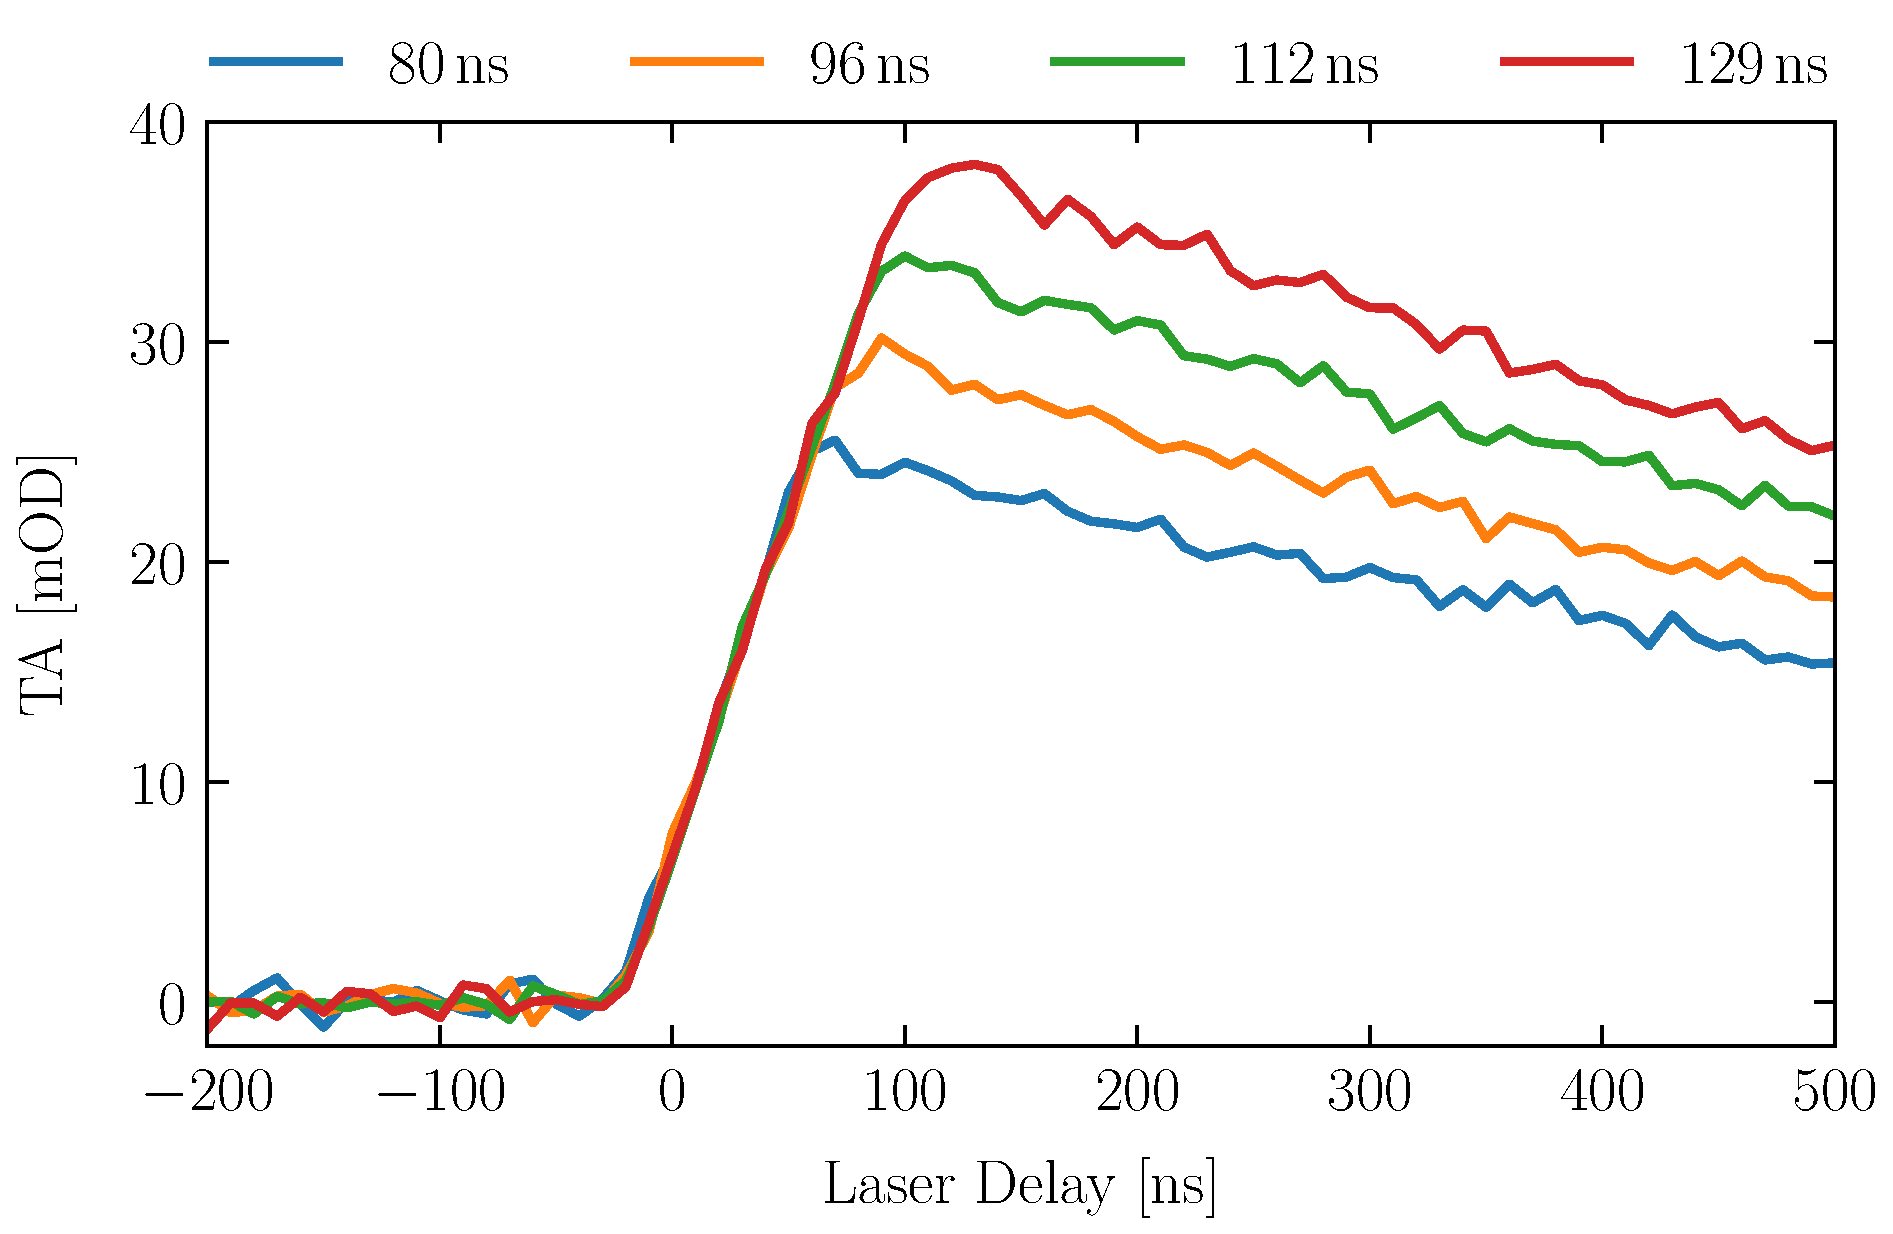
\includegraphics[width = 0.85\textwidth]{Pictures/Evaluation/42/Pump-Laser.pdf}
    \captionof{figure}{
        Transient absorption signal for different pump laser widths using ZnTPP in BN 0.8\,mM.
    }
    \label{fig:pumpLaser}
\end{center}

To investigate the influence of the pump laser width on the transient absorption (TA) signal, we measured for sample 1 [Tab. \ref{tab:lifetimeDecay}] the TA using four different pump laser widths. The TA signal is displayed in Fig. \ref{fig:pumpLaser}. In Fig. \ref{fig:pumpLaser} one can see that there is a shift in the TA maxima which correspond with the set pump laser width. This follows our expectations, since the longer pump laser should be able to exite more electrons to the triplet state. A closer look also shows that the pump laser width has no influnce on the decay rate $k_0$, i.e., the lifetime $\tau$. But to be sure a longer time interval has to be measured to determine the long time behaviour of the decay process.

% etc.

    % 5.Chapter Closure
    % 5. Closure

\chapter{Closure}
\label{chap:close}

    % Appendix
    %% Appendix

\appendix

% Text

% Appendix A

\chapter{Append A}
\label{chap:AppendA}

\section{Append A}


    % Literatur
    \bibliographystyle{Bibliography.bst}
    \bibliography{Bibliography.bib}
    
\end{document}